% Korelasi antar-subtes UTBK-SNBT 2026
% Satu kolom, bahasa Indonesia, abstrak ID & EN.
\documentclass[letterpaper, 12pt]{article}
% Paket dan format naskah: satu kolom, gaya APA 7.

% Ukuran kertas: APA 7 memakai US Letter (8,5 x 11 inci), margin 1 inci.
% Ganti ke a4paper kalau jurnal tujuan meminta A4.
\usepackage[letterpaper,margin=1in]{geometry}

% Encoding dan font
\usepackage[utf8]{inputenc}
\usepackage[T1]{fontenc}
\usepackage{mathptmx}      % mirip Times, termasuk rumus
\usepackage{textcomp}      % simbol tambahan
\usepackage[stretch=30]{microtype}

% Untuk Times New Roman asli: pakai XeLaTeX/LuaLaTeX dan pasang fontnya.
% Nonaktifkan mathptmx, lalu aktifkan dua baris ini:
% \usepackage{fontspec}
% \setmainfont{Times New Roman}

% Bahasa
% Bahasa utama ditaruh terakhir.
\usepackage[english,indonesian]{babel}
% Untuk teks Inggris:
%   \begin{otherlanguage}{english} ... \end{otherlanguage}

% Spasi dan paragraf
\usepackage{setspace}
\doublespacing                       % spasi ganda
\raggedbottom % jangan regangkan isi halaman yang pendek
\usepackage{indentfirst}
\setlength{\parindent}{1.27cm}       % inden 0.5 inci
\setlength{\parskip}{0pt}

% Jangan penggal kata; longgarkan jarak agar teks tetap masuk margin.
\hyphenpenalty=10000
\exhyphenpenalty=10000
\setlength{\emergencystretch}{3em}

% Judul bagian, gaya APA 7
\usepackage{titlesec}
\setcounter{secnumdepth}{0}          % tanpa nomor bagian

% Level 1 -> tengah, tebal
\titleformat{\section}
  {\centering\bfseries\fontsize{12}{14}\selectfont}{}{0em}{}
\titlespacing{\section}{0pt}{*3}{*1.5}

% Level 2 -> rata kiri, tebal
\titleformat{\subsection}
  {\bfseries\fontsize{12}{14}\selectfont}{}{0em}{}
\titlespacing{\subsection}{0pt}{*2.5}{*1}

% Level 3 -> rata kiri, tebal-miring
\titleformat{\subsubsection}
  {\bfseries\itshape\fontsize{12}{14}\selectfont}{}{0em}{}
\titlespacing{\subsubsection}{0pt}{*2}{*0.8}

% Level 4 -> inden, tebal, menyatu dengan paragraf, pakai titik
\titleformat{\paragraph}[runin]
  {\bfseries\fontsize{12}{14}\selectfont}{}{0em}{}[.\ ]
\titlespacing{\paragraph}{1.27cm}{*1.5}{1em}

% Level 5 -> seperti level 4, tapi tebal-miring
\titleformat{\subparagraph}[runin]
  {\bfseries\itshape\fontsize{12}{14}\selectfont}{}{0em}{}[.\ ]
\titlespacing{\subparagraph}{1.27cm}{*1.5}{1em}

% Header: judul pendek dan nomor halaman
\usepackage{fancyhdr}
\pagestyle{fancy}
\fancyhf{}
\newcommand{\runninghead}[1]{\fancyhead[L]{\footnotesize\MakeUppercase{#1}}}
\fancyhead[R]{\footnotesize\thepage}
\renewcommand{\headrulewidth}{0pt}
\setlength{\headheight}{14pt}

% Tabel, gambar, dan caption
\usepackage{graphicx}
\usepackage{float}
\floatplacement{table}{H}
\usepackage{booktabs}
\usepackage{array}
\usepackage{multirow}
\usepackage{caption}
\captionsetup{labelfont=bf, labelsep=period, justification=raggedright,
              singlelinecheck=false, font=small}
\captionsetup[table]{position=above}   % judul di atas tabel

\usepackage{etoolbox}
\AtBeginEnvironment{tabular}{\small}
\setlength{\tabcolsep}{4pt}
\let\origresizebox\resizebox
\renewcommand{\resizebox}[3]{%
  \origresizebox{\ifdim\width>#1 #1\else\width\fi}{#2}{#3}}
% Paksa label bahasa Indonesia meski english jadi bahasa utama TeX.
\renewcommand{\tablename}{Tabel}
\renewcommand{\figurename}{Gambar}

% Rumus dan simbol
\usepackage{amsmath}
\usepackage{amssymb}
\usepackage{icomma}      % koma desimal tanpa spasi ekstra di mode matematika ($0,425$)

% Daftar
\usepackage{enumitem}
\setlist{noitemsep, topsep=4pt}

% Sitasi dan daftar pustaka, gaya APA 7
% Perlu biblatex-apa dan biber.
\usepackage{csquotes}
% Pakai label bibliografi Inggris; naskah tetap bahasa Indonesia.
\DeclareQuoteAlias{english}{indonesian}
\usepackage[
  style=apa,
  backend=biber,
  sorting=nyt,
  sortcites=true,
  uniquename=false,
  uniquelist=false
]{biblatex}
\addbibresource{references.bib}
% Petakan locale Indonesian ke modul english-apa (indonesian-apa.lbx tidak ada).
\DeclareLanguageMapping{indonesian}{english-apa}

% Padanan Indonesia pada sitasi APA 7: "et al." menjadi "dkk." dan "and" pada
% sitasi naratif menjadi "dan" ("&" tetap dipakai pada sitasi dalam kurung).
\DefineBibliographyStrings{english}{andothers = {dkk\adddot}, and = {dan}}
\DefineBibliographyStrings{indonesian}{andothers = {dkk\adddot}, and = {dan}}

% Contoh sitasi:
%   \autocite{key}      -> (Penulis, Tahun)
%   \textcite{key}       -> Penulis (Tahun)
%   \parencite{key}       -> (Penulis, Tahun)
%   \autocite[hlm.\ 12]{key} -> (Penulis, Tahun, hlm. 12)
%
% Aturan APA 7: bila nama penulis menjadi bagian kalimat, tulis nama hanya lewat
% \textcite (Penulis (Tahun), dua penulis "A dan B (Tahun)", tiga atau lebih "A dkk. (Tahun)").
% Bila nama tidak disebut, pakai \autocite atau \parencite ((Penulis, Tahun), dua penulis
% "(A & B, Tahun)"). Jangan menulis nama penulis secara manual di samping sitasi.

% Tautan
% URL panjang boleh pindah baris tanpa tanda hubung.
\usepackage{xurl}
\usepackage[hidelinks]{hyperref} % tanpa kotak warna
\usepackage{orcidlink} % Loads the ORCID link package
\urlstyle{same}

% Longgarkan spasi daftar pustaka untuk DOI/URL panjang.
\AtBeginBibliography{%
  \sloppy
  \setlength{\emergencystretch}{3em}%
}

% Warna
\usepackage{xcolor}   % untuk menandai revisi

% Judul pendek untuk header
\runninghead{Korelasi Antarsubtes UTBK-SNBT 2026}

\begin{document}
\raggedright                         % APA 7: rata kiri, tepi kanan tidak rata
\setlength{\parindent}{1.27cm}       % pulihkan inden setelah \raggedright

\vspace*{3\baselineskip}              % APA 7: judul 3--4 baris dari tepi atas
\begin{center}
  {\bfseries\fontsize{12}{15}\selectfont
  Seberapa Kuat Subtes UTBK-SNBT 2026 Saling Berkorelasi? Estimasi dari Data \textit{Crowdsourced} dan Implikasinya bagi Estimasi Peringkat Nasional\par}

  \vspace{2mm}

  \begin{otherlanguage}{english}
    {\bfseries\fontsize{12}{15}\selectfont
    How Strongly Correlated Are the Subtests in the 2026 Indonesian University Entrance Exam (UTBK-SNBT)? Crowdsourced Estimates and Implications for National Ranking\par}
  \end{otherlanguage}

  \vspace{\baselineskip}

  Galuh Saputra\par
  Peneliti Independen\par
\end{center}

% Catatan Penulis (APA 7: di halaman judul; paragraf 1 ORCID, paragraf 2 ketersediaan kode, ucapan terima kasih,
% dan pengungkapan penggunaan AI, paragraf 3 korespondensi)
\section*{Catatan Penulis}

Galuh Saputra\,\orcidlink{0009-0009-7845-8015} \url{https://orcid.org/0009-0009-7845-8015}

Kode analisis dan materi pendukung paper ini tersedia di \url{https://osf.io/XXXXX}. Penulis berterima kasih kepada Yola Febriani yang ikut mengumpulkan data skor yang tersebar dan kepada para kontributor anonim yang membagikan skor UTBK-SNBT 2026 mereka secara publik. Penulis juga berterima kasih kepada pengelola akun X @sbmptnfess dan @utbkcak yang secara tidak langsung menjadi sumber data paper ini.

Hasil paper ini juga tersedia sebagai kalkulator perkiraan peringkat yang gratis di \url{https://galuhsm.github.io/utbk-correlation-study/}.

Penulis menggunakan Claude (Anthropic) untuk menyunting bahasa dan struktur kalimat agar lebih mudah dipahami pembaca awam, khususnya pembaca seusia peserta UTBK-SNBT, dan untuk mensimulasikan \textit{peer review} guna meningkatkan ketelitian ilmiah. Seluruh isi, analisis, dan keputusan akademik dalam paper ini tetap menjadi tanggung jawab penuh penulis.

Korespondensi mengenai paper ini dapat ditujukan melalui email galmei.id@gmail.com

% Abstrak ID & EN dan kata kunci
\newpage
% Abstrak ID & EN dan kata kunci

\section*{Abstrak}
\noindent
Matriks korelasi antarsubtes Ujian Tertulis Berbasis Komputer--Seleksi Nasional Berdasarkan Tes (UTBK-SNBT) 2026 tidak tersedia bagi publik. Statistik deskriptif per subtes yang beredar bersumber dari tabel internal Panitia Seleksi Nasional Penerimaan Mahasiswa Baru (SNPMB) yang tidak resmi dan belum terverifikasi, sehingga disebut parameter nasional tidak resmi. Penelitian ini bertujuan mengestimasi struktur korelasi kedelapan subtes dengan data \textit{crowdsourced} dari platform X ($N = 1.886$), sekaligus mengidentifikasi karakteristik bias pada metode itu serta implikasinya bagi estimasi peringkat nasional. Rerata korelasi \textit{off-diagonal} pada \textit{raw sample} sebesar $0,300$ tergolong moderat-rendah untuk serangkaian tes kemampuan kognitif yang saling berkaitan. Perbandingan dengan parameter nasional tidak resmi menunjukkan bias seleksi ke arah skor tinggi yang mengindikasikan \textit{restriction of range}. Koreksi Thorndike Case III berbasis iterasi titik tetap pada \textit{pipeline} komputasi terbuka R menghasilkan estimasi korelasi populasi terkoreksi $\bar{R} \approx 0,425$ ($S_Z \approx 67,72$; interval \textit{bootstrap} 95\% untuk $\bar{R}$ $[0,407; 0,442]$). Estimasi ini peka terhadap simpangan baku nasional tidak resmi, karena perubahan seluruh simpangan baku sebesar $\pm 10\%$ menggeser $\bar{R}$ menjadi $0,300$--$0,519$. Distribusi skor nasional juga menyimpang dari normal (miring ke kanan dengan ekor kiri terpotong), dan simulasi menunjukkan bahwa asumsi normal mengubah persentil terutama di ekor distribusi. \textit{Confirmatory factor analysis} (CFA) menunjukkan bahwa model dua faktor (Literasi dan Numerasi) lebih sesuai daripada model dengan satu \textit{g-factor} (\textit{Comparative Fit Index} $0,967$ berbanding $0,932$; $\Delta\chi^2 = 91,55$, $p < 0,001$; korelasi antarfaktor $\phi = 0,813$). Hasil analisis juga mengindikasikan bahwa bias audiens platform tidak dapat diatasi semata-mata melalui \textit{framing} pengumpulan data yang lebih inklusif.

\textit{Kata kunci:} UTBK-SNBT, korelasi antarsubtes, psikometri pendidikan, bias seleksi, data \textit{crowdsourced}, Thorndike Case III, analisis sensitivitas

\newpage

\begin{otherlanguage}{english}
\section*{Abstract}
\noindent
The inter-subtest correlation matrix of the 2026 Indonesian university entrance examination (UTBK-SNBT) is not publicly available, and the subtest-level descriptive statistics in circulation derive from an unofficial, unverified internal table attributed to the national admissions board (SNPMB). This study aims to estimate the correlation structure across the eight subtests of the 2026 UTBK-SNBT using crowdsourced score data from platform X ($N = 1,886$), whilst identifying the characteristics of methodological bias inherent in this approach and the implications for national ranking estimation. The observed raw off-diagonal mean correlation was $0.300$, which is moderate-to-low for a set of interrelated cognitive ability tests. Comparison with these unofficial national parameters indicates a selection bias towards higher scores, consistent with restriction of range. A Thorndike Case III adjustment via fixed-point iteration within an open-source R computational pipeline yielded a corrected population correlation of $\bar{R} \approx 0.425$ ($S_Z \approx 67.72$; 95\% bootstrap interval for $\bar{R}$ $[0.407, 0.442]$). This estimate is sensitive to the unofficial national standard deviations, as changing all of them by $\pm 10\%$ shifts $\bar{R}$ to between $0.300$ and $0.519$. The national score distribution also departs from normality (right-skewed with a truncated left tail), and simulation shows that the normality assumption mainly alters percentiles in the distribution tails. A confirmatory factor analysis showed that a two-factor model (Literacy and Numeracy) fit better than a single general-factor model (CFI $0.967$ versus $0.932$; $\Delta\chi^2 = 91.55$, $p < 0.001$; $\phi = 0.813$). Furthermore, the results indicate that platform-audience bias cannot be resolved solely through more inclusive data-collection framing.

\textit{Keywords:} UTBK-SNBT, inter-subtest correlation, educational psychometrics, selection bias, crowdsourced data, Thorndike Case III, sensitivity analysis
\end{otherlanguage}
\newpage

% Isi naskah
% Pendahuluan
\section{Pendahuluan}

Ujian Tertulis Berbasis Komputer--Seleksi Nasional Berdasarkan Tes (UTBK-SNBT) 2026 mengukur kemampuan peserta melalui delapan skor subtes. Kedelapan skor itu adalah Penalaran Umum (PU), Pengetahuan dan Pemahaman Umum (PPU), Pemahaman Bacaan dan Menulis (PBM), Pengetahuan Kuantitatif (PK), dua skor Literasi dalam Bahasa Indonesia (LBI), yaitu LBI Saintek dan LBI Soshum, Literasi dalam Bahasa Inggris (LBE), dan Penalaran Matematika (PM).

Statistik deskriptif tiap subtes beredar di media sosial dalam bentuk tabel. Isinya meliputi nilai minimum, kuartil pertama, median, rerata, simpangan baku, kuartil ketiga, dan nilai maksimum. Tabel itu disebut berasal dari materi internal Panitia Seleksi Nasional Penerimaan Mahasiswa Baru (SNPMB), tetapi keasliannya belum diverifikasi secara resmi (lihat Bagian Metode). Oleh karena itu, paper ini menyebut tabel itu \textit{parameter nasional tidak resmi (belum terverifikasi)}. Selain itu, parameter itu tidak mencakup informasi mengenai struktur atau matriks korelasi antarsubtes.

Korelasi menunjukkan seberapa kuat skor suatu subtes berkaitan dengan skor subtes lain. Tanpa informasi korelasi, peserta sulit mengetahui persentil skor kompositnya secara nasional. Skor komposit adalah rerata kedelapan skor subtes, sedangkan persentil menunjukkan persentase peserta yang berskor lebih rendah. Persentil tersebut tidak dapat dihitung hanya dari statistik deskriptif per subtes yang tersedia bagi publik. Hal itu terjadi karena simpangan baku skor komposit, yaitu ukuran sebaran skornya, bergantung langsung pada korelasi antarsubtes pembentuknya.

Data korelasi yang belum tersedia ini juga menyisakan persoalan teoretis dalam psikometri pendidikan. Literatur kemampuan kognitif telah lama mendokumentasikan bahwa skor berbagai tes kognitif cenderung bergerak searah atau berkorelasi positif \autocite{spearman1904,carroll1993,jensen1998}. Pola ini dikenal sebagai \textit{positive manifold} dan lazim dikaitkan dengan satu kemampuan umum yang melandasi berbagai tes, yaitu \textit{g-factor}. Selain \textit{g-factor}, \textit{Carroll's three-stratum theory} \autocite{carroll1993} mengidentifikasi faktor kelompok (\textit{group factors}) pada strata di bawahnya, misalnya kemampuan verbal dan kuantitatif. Dengan demikian, struktur korelasi antarsubtes kognitif berpotensi bersifat hierarkis.

Sejauh penelusuran penulis, belum ada studi empiris atau dokumen resmi yang memublikasikan struktur korelasi antarsubtes UTBK-SNBT, baik pada 2026 maupun pada tahun sebelumnya. Celah literatur ini penting karena UTBK-SNBT menjadi tolok ukur seleksi bagi ratusan ribu peserta setiap tahun. Penelitian ini bertujuan mengisi celah tersebut dengan mengestimasi korelasi antarsubtes UTBK-SNBT 2026. Estimasi memanfaatkan data \textit{crowdsourced}, yaitu skor yang dibagikan secara sukarela oleh banyak peserta di platform media sosial X.

Pembagian skor secara sukarela dapat menyempitkan rentang skor sampel teramati dibandingkan populasi (\textit{restriction of range}), sehingga korelasi sebelum koreksi (\textit{raw sample}) cenderung lebih lemah. Korelasi \textit{raw sample} itu dikoreksi dengan Thorndike Case III, yaitu formula untuk seleksi yang terjadi pada skor komposit, sehingga menghasilkan korelasi populasi terkoreksi. Pendekatan ini memiliki sejumlah keterbatasan metodologis, yang diuraikan secara terbuka pada Bagian Metode dan Keterbatasan Penelitian. Meskipun demikian, hasilnya tetap berupa estimasi empiris awal yang penting selama data populasi resmi tidak tersedia bagi publik.

\subsection{Rumusan Masalah}
Berdasarkan latar belakang di atas, penelitian ini merumuskan empat pertanyaan. Pertama, berapa estimasi rerata korelasi antardelapan subtes UTBK-SNBT 2026 berdasarkan data yang tersedia secara publik di media sosial? Kedua, sejauh mana pengambilan sampel dari media sosial menghasilkan estimasi yang bias, yakni menyimpang secara sistematis dari nilai populasi, dan ke mana arah bias itu? Ketiga, apakah kedelapan subtes membentuk satu \textit{g-factor} tunggal atau struktur berjenjang dengan faktor kelompok? Keempat, bagaimana implikasi estimasi korelasi tersebut terhadap penghitungan persentil skor komposit secara nasional?

\subsection{Tujuan Penelitian}
Sejalan dengan keempat pertanyaan tersebut, penelitian ini bertujuan mengestimasi rerata korelasi antardelapan subtes UTBK-SNBT 2026. Tujuan kedua adalah mengidentifikasi arah dan besaran bias akibat pengambilan sampel dari media sosial. Tujuan ketiga adalah menguji struktur faktor kedelapan subtes melalui \textit{confirmatory factor analysis (CFA)}. Tujuan keempat adalah menganalisis implikasi estimasi korelasi itu bagi penghitungan persentil skor komposit secara nasional.

\subsection{Kontribusi Penelitian}
Penelitian ini memberikan tiga kontribusi utama. Kontribusi substantifnya adalah estimasi empiris awal struktur korelasi antarsubtes UTBK-SNBT 2026, yang hingga kini belum tersedia dalam literatur publik, beserta catatan batasan metodologis yang eksplisit. Kontribusi strukturalnya adalah analisis struktur faktor kedelapan subtes melalui CFA. Kontribusi metodologisnya adalah studi kasus tentang dinamika bias seleksi pada data \textit{crowdsourced} media sosial. Studi kasus ini mengindikasikan bahwa perluasan \textit{framing} (cara menyusun ajakan pengumpulan data) agar lebih inklusif belum tentu mengoreksi bias bila audiens platform sumber data telah tersaring secara sosial. Temuan ini menjadi catatan metodologis penting bagi riset pendidikan berbasis \textit{crowdsourcing} di Indonesia.
% Tinjauan pustaka
\section{Tinjauan Pustaka}

\subsection{Struktur Tes UTBK-SNBT 2026}
Setiap subtes UTBK-SNBT 2026 dilaporkan pada skala standar dengan rerata populasi $M = 500$. Khusus LBI, sertifikat 2026 memuat dua nilai sebagai tanggapan atas anggapan bahwa peserta berlatar saintek lebih diuntungkan ketika memilih program studi soshum \autocite{detik2026lbi}. Statistik deskriptif univariat nasional yang dipakai dalam paper ini berasal dari parameter nasional tidak resmi (belum terverifikasi). Asal dan keterbatasannya diuraikan pada Bagian Metode.

\subsection{Korelasi Antarkemampuan Kognitif (\textit{Positive Manifold})}
\textcite{spearman1904} pertama kali mendokumentasikan \textit{positive manifold}, fenomena mendasar dalam kajian kemampuan kognitif. Analisis ulang atas lebih dari 460 kumpulan data \autocite{carroll1993} melahirkan \textit{Carroll's three-stratum theory}, yang menempatkan \textit{g-factor} pada strata tertinggi. Tinjauan komprehensif \textcite{jensen1998} semakin memperkuat landasan teoretis eksistensi \textit{g-factor}. Besaran rerata korelasi antarsubtes yang tersirat dari model semacam ini bergantung pada komposisi rangkaian tes (\textit{test battery}) dan karakteristik sampel. Oleh karena itu, penulis tidak menetapkan rentang acuan numerik apriori.

Selain rerata korelasi tunggal, kerangka faktor kelompok dalam \textit{Carroll's three-stratum theory} \autocite{carroll1993} menyiratkan bahwa subtes kognitif berpotensi membentuk dimensi laten (kemampuan yang tidak diukur langsung) yang lebih spesifik di bawah \textit{g-factor}. Contohnya pembedaan antara kemampuan verbal dan kuantitatif. Pengujian formal terhadap struktur multifaktor semacam ini lazim dilakukan melalui CFA \autocite{brown2015cfa}. CFA membandingkan kecocokan statistik antara \textit{g-factor} tunggal dan model berjenjang yang memuat faktor kelompok spesifik.

\subsection{Penelitian Terdahulu dan Celah Penelitian}
Berbagai bukti empiris berskala besar mendukung korelasi positif antarsubtes tes kognitif. \textcite{jintelligence2026} menghimpun puluhan ribu koefisien korelasi dari ratusan rangkaian tes kognitif dan akademik terstandardisasi. Hasil itu sejalan dengan meta-analisis struktural \textcite{consensusmodel2026} pada domain hubungan kognitif-membaca. Pada tingkat instrumen tunggal, \textcite{waisiv2013} melaporkan korelasi antarsubtes yang moderat pada \textit{Wechsler Adult Intelligence Scale} (WAIS-IV).

Sebagai kasus pembanding yang relevan, studi validitas nasional College Board \autocite{westrick2019} melibatkan 223.858 mahasiswa di 171 perguruan tinggi empat tahun. Studi itu melaporkan korelasi antara skor seksi \textit{Evidence-Based Reading and Writing} dan Matematika pada SAT, yang strukturnya menyerupai komponen literasi dan kuantitatif pada UTBK-SNBT. Korelasi tersebut sebesar $0,58$ pada \textit{raw sample} dan $0,78$ setelah dikoreksi untuk \textit{restriction of range} multivariat terhadap populasi pengikut SAT nasional. Selisih kedua nilai itu muncul pada sampel mahasiswa yang sudah terseleksi dan menunjukkan bahwa \textit{restriction of range} menekan korelasi yang teramati secara substansial.

Sejauh penelusuran pustaka yang dilakukan, belum ditemukan publikasi ilmiah maupun laporan resmi yang menyajikan struktur korelasi antarsubtes UTBK-SNBT secara spesifik. Dengan demikian, paper ini diposisikan untuk mengisi celah informasi empiris itu.

\subsection{Kerangka Berpikir}
Paper ini bersifat eksploratif-deskriptif, sehingga hipotesis statistik formal tidak dirumuskan. Istilah konfirmatori pada CFA merujuk pada teknik pembandingan model faktor. Sintesis literatur psikometri di atas mengarah pada satu ekspektasi kualitatif. Apabila UTBK-SNBT memiliki karakteristik pengukuran yang serupa dengan rangkaian tes kognitif terstandardisasi lainnya, korelasi antarsubtesnya diperkirakan positif secara konsisten. Apabila korelasi pada \textit{raw sample} ternyata relatif lemah dan disertai indikasi \textit{restriction of range} pada parameter sampel teramati (sebagaimana dipaparkan pada Bagian Hasil), kondisi itu diposisikan sebagai indikasi awal bias metodologis dalam pengambilan sampel. Kondisi itu tidak ditafsirkan sebagai cerminan struktur psikometri UTBK-SNBT yang berbeda secara mendasar dari tes kognitif pada umumnya.

Kerangka faktor kelompok pada \textit{Carroll's three-stratum theory} juga mengarah pada ekspektasi struktur faktor yang berjenjang. Dalam struktur itu, domain Literasi (verbal) dan Numerasi (kuantitatif) menjadi dua faktor kelompok di bawah \textit{g-factor}. CFA membandingkan ekspektasi tersebut dengan \textit{g-factor} tunggal.
% Metode
\section{Metode}

\subsection{Desain Penelitian}
Paper ini memakai desain deskriptif-korelasional noneksperimental dan tidak mengumpulkan data melalui instrumen primer. Data yang dipakai bersifat sekunder, yaitu skor yang dibagikan secara sukarela oleh peserta UTBK-SNBT 2026 di media sosial X. Estimasi korelasi antarsubtes dihitung dari sampel teramati. Statistik deskriptif sampel, yaitu rerata dan simpangan baku ($SD$), kemudian dibandingkan dengan parameter nasional tidak resmi (belum terverifikasi) untuk menilai sejauh mana sampel mencerminkan populasi sasaran.

\subsection{Sumber Data}
Parameter nasional tidak resmi (belum terverifikasi) yang dipakai sebagai pembanding (Tabel~\ref{tab:deskriptif}) tidak bersumber langsung dari kanal resmi SNPMB. Tabel itu diperoleh dari unggahan di platform X sekitar 8 jam setelah pengumuman skor peserta SNBT 2026. Menurut klarifikasi akun @\textcite{kevins2026}, yang narasi unggahannya mengindikasikan keterlibatan internal kepanitiaan SNPMB walaupun tidak dicantumkan pada profil akun, data itu semula disiapkan untuk materi konferensi pers, tetapi batal ditayangkan atas keputusan rapat internal tanpa penjelasan publik.

Triangulasi independen dilakukan untuk menguji keaslian data itu dengan membandingkan sejumlah nilai ekstrem pada tabel terhadap skor yang diunggah secara mandiri oleh peserta. Hasilnya menunjukkan kesesuaian pada beberapa sampel, seperti skor PK tertinggi sebesar 1.173,55 pada peserta yang diterima di STEI-K ITB dan skor PM tertinggi sebesar 997,70 pada peserta di FTI-RI ITB. Presisi angka yang tinggi dan jeda waktu kemunculan data yang relatif singkat memperkuat dugaan bahwa data itu asli. Namun, triangulasi ini bersifat parsial. Pengujian hanya mencakup dua nilai ekstrem, sedangkan rerata, simpangan baku, dan kuartil belum teruji. Nilai $M = 500$ yang seragam pada seluruh subtes mengikuti definisi skala sehingga tidak informatif sebagai bukti keaslian. Atas dasar itu, tabel ini tetap disebut parameter nasional tidak resmi (belum terverifikasi), dan status perolehannya dicatat secara terbuka pada Bagian Keterbatasan Penelitian.

Berbeda dengan tabel itu, jumlah peserta hadir pada UTBK-SNBT 2026 ($N_{\text{nasional}} = 846.518$, dari 871.496 pendaftar) bersumber dari paparan resmi konferensi pers hasil SNBT 2026 yang dipublikasikan \textcite{snpmb2026konferensi}. Angka ini hanya dipakai untuk menghitung peringkat nasional dan jumlah peserta yang diharapkan berada di luar rentang skor.

Skor pada kedelapan komponen UTBK-SNBT 2026 dihimpun dari unggahan publik di platform X, terutama melalui akun @sbmptnfess dan @utbkcak. Pada akun @sbmptnfess, data dijaring dari utas khusus perguruan tinggi negeri (PTN) tertentu, seperti Institut Teknologi Bandung (ITB), Universitas Brawijaya (UB), Universitas Gadjah Mada (UGM), dan Universitas Indonesia (UI). Data juga dijaring dari utas terbuka yang mengundang pembagian nilai tanpa membatasi status kelulusan. Seluruh data yang dianalisis berupa tangkapan layar sertifikat resmi hasil ujian yang diunggah langsung oleh peserta.

\subsection{Prosedur Pengumpulan Data}
Pengumpulan data berlangsung dalam tiga langkah yang mencakup 19 klaster utas. Pertama, penyisiran utas bertema PTN tertentu di akun @sbmptnfess menjaring $N = 1.459$ entri. Kedua, perluasan ke utas umum pada akun @sbmptnfess menambah jumlah entri menjadi $N = 1.709$. Ketiga, penambahan dari akun @utbkcak menggenapkan total sampel menjadi $N = 1.886$ setelah prosedur pembersihan (lihat Subbagian Pembersihan dan Validasi Data). Tiap penambahan klaster disebut tahap (Tahap 1 sampai 19) pada Bagian Hasil. Bagian itu juga menyajikan tren estimasi korelasi, yang berfluktuasi lalu melandai (\textit{plateau}) seiring penambahan tahap.

\subsection{Variabel Penelitian}
Paper ini menganalisis kedelapan skor subtes UTBK-SNBT 2026, yaitu PU, PPU, PBM, PK, LBI Saintek, LBI Soshum, LBE, dan PM. Skor komposit dihitung sebagai rerata aritmetis kedelapan skor subtes, $Z = \frac{1}{8}\sum_{k=1}^8 X_k$, untuk menyusun matriks translasi persentil standar, tabel yang menerjemahkan titik persentil standar ($M \pm k\,SD$) menjadi skor (lihat Bagian Hasil). LBI Saintek dan LBI Soshum diperlakukan sebagai dua komponen mandiri dengan bobot setara terhadap enam subtes lain, tanpa digabung lebih dahulu menjadi satu nilai.

LBI diujikan sebagai satu tes yang sama bagi seluruh peserta \autocite{detik2026lbi}, sedangkan pada tahun-tahun sebelumnya LBI dilaporkan sebagai satu nilai. Sejauh penelusuran penulis, prosedur Panitia SNPMB menurunkan dua skor dari satu tes itu belum dijelaskan secara terbuka. Dengan demikian, LBI Saintek dan LBI Soshum merupakan dua skor dari satu tes pada peserta yang sama dan tidak independen secara desain. Pada skor komposit, LBI memperoleh bobot $\frac{2}{8}$, dua kali bobot subtes lain ($\frac{1}{8}$). Penulis mempertahankan spesifikasi ini agar sesuai dengan format sertifikat, dan hasil analisis sensitivitasnya dilaporkan pada Bagian Hasil.

\subsection{Pembersihan dan Validasi Data}
Sebelum korelasi diestimasi, data awal disaring dengan tiga kriteria eksklusi. Kriteria pertama adalah \textbf{duplikasi data}, yaitu entri dengan kombinasi nilai identik pada kedelapan subtes, yang dideteksi melalui pencocokan nilai persis antarentri pada skrip pembersihan data. Kriteria kedua adalah \textbf{nilai di luar rentang}, yaitu entri dengan skor yang melampaui batas minimum atau maksimum nasional tidak resmi pada subtes terkait, sebagai indikasi kesalahan input. Kriteria ketiga adalah \textbf{indikasi manipulasi visual atau rekayasa kecerdasan buatan}, yang mencakup (a) keberadaan \textit{watermark} generator kecerdasan buatan pada gambar sertifikat, (b) nilai bulat sempurna, seperti skor tepat 1.000,00, yang tidak mungkin muncul pada penskalaan \textit{Item Response Theory} (IRT), dan (c) ketidakkonsistenan tata letak digit dengan pola sebaran alami sertifikat resmi. Metode IRT menaksir skor dari pola jawaban pada tiap butir soal. Alasannya, skor maksimum nasional PM hanya 997,70, dan PK tidak memiliki riwayat nilai bulat.

Kriteria duplikasi hanya berlaku apabila kedelapan nilai identik sekaligus, sehingga nilai yang sama pada satu subtes saja tidak dianggap duplikasi. Pada LBI Saintek, misalnya, terdapat 1.396 nilai berbeda di antara 1.886 entri (nilai 752,30 muncul 19 kali), tetapi entri-entri itu memiliki profil skor yang berbeda pada tujuh subtes lainnya. Penyebab seringnya nilai kembar pada subtes ini belum ditelusuri.

\subsection{Teknik Analisis Data dan Keterbukaan Replikasi}
Seluruh analisis, estimasi statistik, dan visualisasi dijalankan secara terprogram dengan skrip komputasi terbuka berbahasa pemrograman R versi 4.6.1. Korelasi Pearson teramati dihitung untuk 28 pasangan unik antarsubtes. Rerata korelasi \textit{off-diagonal} (rerata koefisien di luar diagonal matriks korelasi) dihitung dengan membagi jumlah koefisien itu dengan 56, banyak sel di luar diagonal pada matriks $8 \times 8$ ($8^2 - 8 = 56$; Tabel~\ref{tab:korelasi}). Bias seleksi dievaluasi dengan membandingkan rerata dan $SD$ sampel teramati terhadap parameter nasional tidak resmi (Tabel~\ref{tab:deskriptif}).

Penulis memilih formula Thorndike Case III \autocite{thorndike1949,sackett2000} untuk mengoreksi atenuasi (pelemahan korelasi) akibat \textit{restriction of range}. Formula ini merupakan derivasi operasional dari teorema seleksi multivariat Lawley--Aitken \autocite{aitken1934,lawley1943}. Pilihan itu didasarkan pada mekanisme bias sukarela di media sosial yang terjadi langsung pada skor komposit $Z$, sedangkan Case II mengasumsikan seleksi langsung pada salah satu variabel yang dikorelasikan. Akibatnya, korelasi tiap pasangan subtes $X_i$ dan $X_j$ melemah secara tidak langsung (\textit{incidental restriction}), karena seleksi pada $Z$ menjalar ke tiap subtes melalui kovarians keduanya dengan $Z$. Estimasi korelasi populasi terkoreksi ($R_{ij}$) dihitung melalui persamaan:
\begin{equation}
R_{ij} = \frac{r_{ij} + r_{iZ} r_{jZ} \left(\frac{S_Z^2}{s_Z^2} - 1\right)}{\sqrt{\left[1 + r_{iZ}^2 \left(\frac{S_Z^2}{s_Z^2} - 1\right)\right] \left[1 + r_{jZ}^2 \left(\frac{S_Z^2}{s_Z^2} - 1\right)\right]}}
\end{equation}
dengan $r_{ij}$ sebagai korelasi \textit{raw sample}, $r_{iZ}$ dan $r_{jZ}$ sebagai korelasi masing-masing subtes dengan $Z$, $s_Z \approx 53,84$ sebagai $SD$ skor komposit sampel teramati, $S_Z$ sebagai $SD$ skor komposit populasi, dan $\lambda^2 = \frac{S_Z^2}{s_Z^2} - 1$ sebagai multiplikator seleksi (kenaikan relatif varians skor komposit populasi terhadap sampel teramati).

Karena $S_Z$ dan $R_{ij}$ saling bergantung (ketergantungan sirkular), $S_Z$ diestimasi melalui iterasi titik tetap (\textit{fixed-point iteration}), prosedur yang mengulang penghitungan sampai nilainya berhenti berubah. Prosedur ini memakai matriks kovarians heterogen penuh:
\begin{equation}
S_{Z}^{(k+1)} = \sqrt{\frac{1}{64}\left( \sum_{i=1}^8 \sigma_i^2 + \sum_{i=1}^8 \sum_{j \neq i}^8 \sigma_i \sigma_j R_{ij}^{(k)} \right)}
\end{equation}
dengan $\sigma_{\text{PU}} = 71,52$ dan $\sigma_{\text{lain}} = 100,00$ dari parameter nasional tidak resmi (Tabel~\ref{tab:deskriptif}). Iterasi dijalankan pada skrip R dengan toleransi presisi tinggi ($|\Delta S_Z| \le 10^{-12}$), berawal dari $s_Z$, dan mencapai konvergensi stabil pada siklus ke-43.

Agar analisis dapat direproduksi secara komputasi (\textit{computational reproducibility}) dan diperiksa secara terbuka, seluruh kode analisis R, berkas data replikasi tanpa identitas peserta, kamus data (\textit{codebook}), dan skrip pengujian otomatis (\textit{unit tests}) disimpan secara terbuka di repositori riset publik.

\subsection{Analisis Faktor Eksploratori dan Konfirmatori}
Guna menguji apakah kedelapan skor subtes membentuk \textit{g-factor} tunggal atau struktur berjenjang dengan faktor kelompok yang lebih spesifik (lihat Tinjauan Pustaka), penulis menjalankan \textit{exploratory factor analysis} (EFA), yang mencari struktur faktor langsung dari data, dan CFA. Keduanya memakai paket \texttt{psych} \autocite{revelle2024psych} dan \texttt{lavaan} \autocite{rosseel2012lavaan} pada R. \textit{Horn's Parallel Analysis} \autocite{horn1965} dijalankan sebagai diagnostik pendukung. Prosedur ini membandingkan nilai eigen (besar varians yang dijelaskan tiap faktor) matriks korelasi sampel teramati dengan nilai eigen matriks acak hasil simulasi berukuran setara. Penulis menjalankannya berbasis faktor, dengan metode ekstraksi \textit{minres} dan 100 iterasi simulasi. Penulis menetapkan dua faktor pada EFA secara apriori, mengikuti pembedaan domain Literasi dan Numerasi pada kerangka teori (lihat Tinjauan Pustaka), dan tidak semata-mata mengikuti jumlah faktor yang disarankan \textit{Parallel Analysis} (hasilnya dilaporkan pada Bagian Hasil).

Dua model CFA dibandingkan. Model 1 memuat \textit{g-factor} tunggal yang membebani kedelapan subtes dengan muatan yang diestimasi bebas, sedangkan Model 2 memuat dua faktor berkorelasi, yaitu Literasi dan Numerasi, sesuai hasil ekstraksi EFA. Kedua model diestimasi dengan \textit{robust maximum likelihood} (estimator MLM, uji Satorra--Bentler) karena data mengindikasikan sebaran miring dan menyimpang dari normal (lihat Bagian Hasil, Subbagian Evaluasi Asumsi Distribusi). Kecocokan model (kesesuaian antara korelasi yang diturunkan model dan korelasi teramati) dievaluasi melalui $\chi^2_{\text{SB}}$, \textit{Comparative Fit Index} (CFI), \textit{Tucker--Lewis Index} (TLI), \textit{Root Mean Square Error of Approximation} (RMSEA) beserta selang kepercayaan 90\%, \textit{Standardized Root Mean Square Residual} (SRMR), dan \textit{Akaike Information Criterion} (AIC), berdasarkan ambang batas \textcite{hubentler1999}. Keunggulan Model 2 terhadap Model 1 diuji melalui selisih $\chi^2$ berskala (\textit{scaled chi-square difference test}).

\subsection{Analisis Sensitivitas dan Ketidakpastian}
Analisis berikut bersifat tambahan dan tidak mengubah spesifikasi utama, yaitu delapan subtes, CFA dua-faktor apriori, dan $SD$ nasional tidak resmi tanpa penyesuaian.

Pertama, peran LBI sebagai satu tes dengan dua skor diperiksa melalui tiga analisis. Analisis pertama adalah EFA tiga-faktor (ekstraksi \textit{minres}, rotasi \textit{oblimin} yang mengizinkan faktor berkorelasi) untuk menafsirkan faktor ketiga. Analisis kedua adalah CFA dua-faktor dengan kovarians residual (keterkaitan antara LBI Saintek dan LBI Soshum di luar kedua faktor), yang dibandingkan dengan model utama melalui uji selisih $\chi^2$ Satorra--Bentler. Analisis ketiga adalah koreksi Case III yang diulang dengan salah satu atau kedua skor LBI dikeluarkan dari skor komposit. Rerata kedua skor LBI tidak dipakai sebagai satu variabel karena $SD$ nasionalnya tidak tersedia.

Kedua, ketidakpastian pengambilan sampel (variasi estimasi akibat sampel yang ditarik berbeda) diperkirakan dengan \textit{bootstrap} nonparametrik, yang menarik ulang entri secara acak dari sampel teramati. Sebanyak 2.000 sampel \textit{bootstrap} ditarik dengan pengembalian dari seluruh entri sampel teramati (benih acak 2026). Pada tiap sampel \textit{bootstrap}, korelasi \textit{raw sample}, korelasi subtes-komposit, dan $SD$ skor komposit dihitung ulang sebelum iterasi titik tetap dijalankan sampai konvergen. Interval persentil 95\% dilaporkan untuk $S_Z$, $\lambda^2$, dan $\bar{R}$. \textit{Bootstrap} hanya menangkap ketidakpastian pengambilan sampel.

Ketiga, ketidakakuratan $SD$ nasional diuji dengan mengulang estimasi utama pada seluruh entri sampel teramati setelah seluruh $SD$ nasional dikalikan $0,90$; $0,95$; $1,05$; atau $1,10$. Pengulangan juga dilakukan setelah $SD_{\text{PU}}$ diganti $100$ dengan $SD$ subtes lain tetap.

Keempat, asumsi normalitas yang mendasari translasi persentil diperiksa dalam dua langkah. Langkah pertama adalah diagnostik deskriptif yang dihitung dari tujuh statistik nasional tidak resmi tiap subtes. Diagnostik ini mencakup skor-$z$ minimum dan maksimum, jumlah peserta yang diharapkan berada di luar rentang tersebut pada distribusi normal dengan 846.518 peserta hadir, kemiringan Bowley $\frac{Q_3 + Q_1 - 2\,\text{Med}}{Q_3 - Q_1}$ dengan $Q_1$, Med, dan $Q_3$ sebagai kuartil pertama, median, dan kuartil ketiga, selisih rerata dan median, dan rasio rentang antarkuartil terhadap $SD$ ($\frac{IQR}{SD}$), yang bernilai $1,349$ pada distribusi normal.

Langkah kedua adalah simulasi. Karena data mikro nasional (skor tiap peserta) tidak tersedia, transformasi normalisasi seperti Box-Cox tidak dapat diterapkan. Sebagai gantinya, distribusi marginal tiap subtes (sebaran skor satu subtes secara terpisah) dihampiri distribusi Johnson SB \autocite{johnson1949}. Distribusi berbatas dengan empat parameter ini dapat meniru ekor kiri terpotong dan ekor kanan panjang. Parameter dicocokkan dengan kuadrat terkecil berbobot terhadap tujuh statistik nasional tidak resmi. Skor minimum dan maksimum masing-masing diletakkan pada peluang $\frac{0,5}{N}$ dan $1 - \frac{0,5}{N}$ sebagai hampiran nilai ekstrem pada sampel besar, dan pencarian dimulai dari 40 titik awal acak (benih acak 2026). Skor komposit kemudian disimulasikan untuk 1.000.000 peserta virtual dengan \textit{copula} Gaussian, model yang menghubungkan distribusi marginal melalui satu korelasi laten seragam pada skala normal baku. Simulasi A memakai korelasi laten sebesar $\bar{R}$ hasil Thorndike Case III. Simulasi B memakai korelasi laten yang dikalibrasi agar $SD$ skor komposit simulasi sama dengan $S_Z$, sehingga pengaruh bentuk distribusi terpisah dari pengaruh skala. Skor komposit simulasi dipusatkan ke rerata $500$ karena hampiran marginal menyisakan galat rerata beberapa poin. Hasil simulasi dibandingkan dengan versi normal melalui dua ukuran, yaitu peluang ekor di luar titik $M \pm k\,S_Z$ dan skor komposit simulasi pada persentil yang sama dengan persentil normal di titik tersebut.

Kelima, \textit{Spearman's Law of Diminishing Returns} (SLODR), atau diferensiasi kemampuan, diperiksa melalui model satu faktor. SLODR menyatakan bahwa korelasi antartes lebih rendah pada kemampuan tinggi dan lebih tinggi pada kemampuan rendah. Muatan \textit{g-factor} pada model itu menurun linear terhadap tingkat kemampuan, $m(g) = m_0 - b\,g$ dengan $g \sim N(0,1)$ dan $b \in \{0; 0,01; 0,02; 0,03; 0,04\}$ ($b = 0$ berarti korelasi konstan). Tiap skor laten diubah menjadi normal baku melalui peringkat agar distribusi marginal tidak berubah. Simulasi ini terdiri atas dua bagian. Pada bagian pertama, marginal Johnson SB digunakan dan $m_0$ dikalibrasi agar $SD$ skor komposit sama dengan $S_Z$, lalu peluang ekor dan skor komposit dibandingkan antarskenario dan dengan normal. Pada bagian kedua, populasi Gaussian dengan $SD$ nasional tidak resmi diseleksi lewat skor komposit dengan probabilitas seleksi logistik, yang parameternya dicocokkan ke rerata dan $SD$ skor komposit sampel teramati. Nilai $m_0$ dikalibrasi agar rerata korelasi \textit{raw sample} pada sampel simulasi sama dengan sampel teramati ($b \in \{0; 0,02; 0,04\}$). Prosedur Case III yang sama kemudian dijalankan pada sampel simulasi dan dibandingkan dengan nilai sebenarnya pada populasi simulasi. Simulasi SLODR memakai $300.000$ peserta virtual dan benih acak 2026.

\subsection{Pertimbangan Etis}
Seluruh data yang dianalisis bersumber dari unggahan publik pada platform X yang dapat diakses secara terbuka tanpa autentikasi khusus. Analisis dan pelaporan hasil dilakukan sepenuhnya pada tingkat agregat, tanpa mencantumkan identitas pribadi peserta (nama akun maupun identitas asli) di bagian mana pun dalam paper ini.
% Hasil
\section{Hasil}

\subsection{Perbandingan Statistik Deskriptif Sampel dan Parameter Nasional Tidak Resmi}

\begin{table}[H]
    \centering
    \caption{Perbandingan Statistik Deskriptif Sampel ($N=1.886$) dan Parameter Nasional Tidak Resmi per Subtes}
    \label{tab:deskriptif}
    \begin{spacing}{1.0}
    \begin{tabular}{lcccccc}
        \toprule
        Subtes & $M$ (Sampel) & $SD$ (Sampel) & $M$ (Nasional) & $SD$ (Nasional) & $\Delta M$ & $\Delta SD$ \\
        \midrule
        PU              & 633,26 & 76,85 & 500,00 & 71,52 & 133,26 & 5,33 \\
        PPU             & 669,96 & 61,50 & 500,00 & 100,00 & 169,96 & -38,50 \\
        PBM             & 680,95 & 76,62 & 500,00 & 100,00 & 180,95 & -23,38 \\
        PK              & 678,53 & 131,90 & 500,00 & 100,00 & 178,53 & 31,90 \\
        LBI Saintek     & 631,63 & 82,31 & 500,00 & 100,00 & 131,63 & -17,69 \\
        LBI Soshum      & 634,69 & 70,11 & 500,00 & 100,00 & 134,69 & -29,89 \\
        LBE             & 680,44 & 86,50 & 500,00 & 100,00 & 180,44 & -13,50 \\
        PM              & 653,23 & 100,01 & 500,00 & 100,00 & 153,23 & 0,01 \\
        \bottomrule
    \end{tabular}
    \end{spacing}
    \vspace{2mm}
    \begin{flushleft}
    \footnotesize\textit{Catatan.} $\Delta M = M_{\text{sampel}} - M_{\text{nasional}}$; $\Delta SD = SD_{\text{sampel}} - SD_{\text{nasional}}$. Parameter nasional tidak resmi bersumber dari tabel internal Panitia Seleksi Nasional Penerimaan Mahasiswa Baru (SNPMB) yang beredar di media sosial dan belum terverifikasi secara resmi (triangulasi parsial pada nilai maksimum PK dan PM; lihat Bagian Metode).
    \end{flushleft}
\end{table}


Rerata sampel melampaui rerata nasional sebesar 131,63--180,95 poin pada seluruh subtes (Tabel~\ref{tab:deskriptif}), sehingga sampel ($N=1.886$) condong ke skor tinggi. $SD$ sampel menyusut pada enam dari delapan subtes dibandingkan parameter nasional tidak resmi, dan penyusutan itu mengindikasikan \textit{restriction of range}. Penurunan terbesar teramati pada PPU ($-38,50$ poin) dan LBI Soshum ($-29,89$ poin). Sebaliknya, $SD$ PK membesar 31,90 poin akibat nilai ekstrem sebesar 1.173,55 (dievaluasi pada Subbagian Evaluasi Asumsi Distribusi). Selain itu, hanya 0,42\% sampel yang berada di bawah rerata nasional ($M=500$), jauh dari proporsi 50\% yang diharapkan pada sampel representatif.

\subsection{Evaluasi Asumsi Distribusi}
Tujuh statistik nasional tidak resmi per subtes menunjukkan bahwa distribusi skor menyimpang dari normal (Tabel~\ref{tab:nonnormal_diag}). Skor minimum nasional jauh lebih dekat ke rerata daripada yang diharapkan. Nilai $z$ minimum berkisar dari $-1,43$ (PK) hingga $-2,89$ (LBI Soshum), padahal pada populasi normal berukuran 846.518 peserta hadir minimum diharapkan sekitar $-4,72$ $SD$. Bila distribusi normal, jumlah peserta yang seharusnya berada di bawah minimum nasional berkisar dari sekitar 1.654 (LBI Soshum) hingga 64.760 (PK), sedangkan jumlah teramati sekitar satu. Skor $M - 3\,SD$ berada di bawah minimum nasional pada seluruh subtes. Di sisi atas, $z$ maksimum melampaui batas normal ($4,72$) pada PU ($5,51$), PM ($4,98$), dan PK ($6,74$, skor $1.173,55$), tetapi tidak pada subtes lain ($3,91$ pada LBE hingga $4,54$ pada LBI Saintek). Selisih rerata dan median bernilai positif pada enam subtes (PK $25,1$; LBE $16,3$; PM $10,9$) dan sedikit negatif pada kedua skor LBI ($-3,76$ dan $-3,65$). Kemiringan Bowley terbesar teramati pada PK ($0,26$), sedangkan rasio $\frac{IQR}{SD}$ ($1,33$--$1,54$) berada di sekitar nilai normal ($1,349$). Pola ini berupa distribusi miring ke kanan dengan ekor kiri terpotong dan paling menonjol pada PK, LBE, dan PM.

\begin{table}[H]
    \centering
    \caption{Diagnostik Nonnormalitas Parameter Nasional Tidak Resmi per Subtes}
    \label{tab:nonnormal_diag}
    \begin{spacing}{1.0}
    \resizebox{\textwidth}{!}{%
    \begin{tabular}{lcccccc}
        \toprule
        Subtes & $z$ Minimum & $z$ Maksimum & $N$ Diharapkan $<$ Minimum & Bowley & Rerata$-$Median & $\frac{IQR}{SD}$ \\
        \midrule
        PU & -2,71 & 5,51 & 2.826 & 0,04 & 5,4 & 1,33 \\
        PPU & -2,68 & 4,35 & 3.109 & 0,06 & 4,9 & 1,45 \\
        PBM & -2,70 & 4,41 & 2.917 & 0,03 & 4,9 & 1,39 \\
        PK & -1,43 & 6,74 & 64.760 & 0,26 & 25,1 & 1,36 \\
        LBI Saintek & -2,54 & 4,54 & 4.704 & -0,06 & -3,8 & 1,45 \\
        LBI Soshum & -2,89 & 4,17 & 1.654 & -0,04 & -3,6 & 1,43 \\
        LBE & -1,83 & 3,91 & 28.572 & 0,12 & 16,3 & 1,37 \\
        PM & -2,33 & 4,98 & 8.361 & 0,12 & 10,9 & 1,54 \\
        \bottomrule
    \end{tabular}%
    }
    \end{spacing}
    \vspace{2mm}
    \begin{flushleft}
    \footnotesize\textit{Catatan.} $z = \frac{\text{skor} - 500}{SD}$ nasional. Pada distribusi normal dengan $N_{\text{nasional}} = 846.518$, minimum dan maksimum diharapkan sekitar $\mp 4,72$ $SD$ dari rerata; kemiringan Bowley $= 0$; dan $\frac{IQR}{SD} = 1{,}349$, dengan $IQR$ sebagai rentang antarkuartil. ``$N$ Diharapkan $<$ Minimum'' = $N_{\text{nasional}} \cdot \Phi(z_{\min})$, yaitu jumlah peserta yang seharusnya berada di bawah minimum nasional bila distribusi normal (nilai teramati sekitar satu). Skor $M - 3\,SD$ berada di bawah minimum nasional pada seluruh subtes.
    \end{flushleft}
\end{table}


Dampak ketidaknormalan diperiksa melalui simulasi (Tabel~\ref{tab:nonnormal_sim}). Distribusi Johnson SB \autocite{johnson1949} untuk tiap subtes cocok dengan kuantil, rerata, dan $SD$ nasional (nilai fungsi tujuan $\leq 0,009$ pada semua subtes; galat kuantil umumnya di bawah tiga poin, terbesar $7,5$ poin pada median LBI Saintek, sedangkan galat rerata hingga $5,2$ poin dan galat $SD$ hingga $5,5$ poin). Skor komposit simulasi miring ke kanan (\textit{skewness} $0,41$--$0,42$; ekskurtosis berlebih $0,06$). Simulasi A (korelasi laten $0,425$) menghasilkan $SD$ skor komposit $68,3$, sedangkan simulasi B (korelasi laten $0,415$) menghasilkan $S_Z = 67,72$. Kedua simulasi menghasilkan pola yang sama. Di sekitar $\pm 1\,SD$, hasil simulasi dekat dengan normal (selisih skor kurang dari $1,5$ poin). Di ekor atas, peluang melampaui $M + 2\,S_Z$ adalah $3,44\%$ (A) dan $3,32\%$ (B) dibandingkan $2,28\%$ pada normal, dan peluang melampaui $M + 3\,S_Z$ adalah $0,407\%$ dan $0,380\%$ dibandingkan $0,135\%$. Peringkat nasional setara $M + 3\,S_Z$ berubah dari sekitar 1.143 menjadi 3.216--3.446. Skor komposit pada persentil normal ke-97,7 dan ke-99,9 pada simulasi B adalah $649$ dan $730$, atau $13,4$ dan $26,9$ poin di atas versi normal ($635$ dan $703$). Di ekor bawah, peluang berada di bawah $M - 2\,S_Z$ hanya $0,89\%$ (A) dan $0,83\%$ (B) dibandingkan $2,28\%$, dan peluang di bawah $M - 3\,S_Z$ praktis nol. Skor pada persentil normal ke-2,3 dan ke-0,13 pada simulasi B adalah $381$ dan $343$ dibandingkan $365$ dan $297$.

\begin{table}[H]
    \centering
    \caption{Sensitivitas Persentil dan Skor Komposit terhadap Asumsi Normal dengan Marginal Johnson SB dan \textit{Copula} Gaussian}
    \label{tab:nonnormal_sim}
    \begin{spacing}{1.0}
    \resizebox{\textwidth}{!}{%
    \begin{tabular}{lccccccc}
        \toprule
        & \multicolumn{3}{c}{Peluang Ekor (\%)} & \multicolumn{4}{c}{Skor Komposit pada Persentil Normal} \\
        \cmidrule(lr){2-4} \cmidrule(lr){5-8}
        Titik & Normal & Simulasi A & Simulasi B & Normal & Simulasi A & Simulasi B & Selisih B \\
        \midrule
        $M - 3\,S_Z$ & 0,135 & $<0{,}001$ & $<0{,}001$ & 296,9 & 341,6 & 342,5 & 45,7 \\
        $M - 2\,S_Z$ & 2,275 & 0,891 & 0,834 & 364,6 & 380,2 & 381,1 & 16,5 \\
        $M - 1\,S_Z$ & 15,866 & 16,275 & 16,014 & 432,3 & 431,3 & 431,9 & -0,3 \\
        $M + 1\,S_Z$ & 15,866 & 16,297 & 16,108 & 567,7 & 569,1 & 568,5 & 0,8 \\
        $M + 2\,S_Z$ & 2,275 & 3,439 & 3,325 & 635,4 & 650,2 & 648,8 & 13,3 \\
        $M + 3\,S_Z$ & 0,135 & 0,407 & 0,380 & 703,1 & 732,3 & 730,1 & 26,9 \\
        \bottomrule
    \end{tabular}%
    }
    \end{spacing}
    \vspace{2mm}
    \begin{flushleft}
    \footnotesize\textit{Catatan.} Skor komposit adalah rerata delapan subtes, dengan 1.000.000 peserta virtual. Marginal tiap subtes dihampiri distribusi Johnson SB yang dicocokkan ke kuantil, rerata, dan $SD$ nasional tidak resmi, dan dependensi dimodelkan dengan \textit{copula} Gaussian berkorelasi seragam. Simulasi A memakai korelasi laten $= 0,425$ ($\bar{R}$ Thorndike) dan menghasilkan $SD$ skor komposit $= 68,3$. Simulasi B memakai korelasi laten $= 0,415$, dikalibrasi agar $SD$ skor komposit $= S_Z = 67,72$. Skor komposit simulasi dipusatkan ke rerata $500$ (pergeseran 2,39 poin). Titik $M \pm k\,S_Z$ dengan $M = 500$. Peluang ekor mengacu pada sisi bawah untuk $k<0$ dan sisi atas untuk $k>0$. Selisih B = skor simulasi B $-$ skor normal.
    \end{flushleft}
\end{table}


Estimasi korelasi dan translasi persentil pada Tabel~\ref{tab:ranking_subtes} dan~\ref{tab:ranking_komposit} tetap menggunakan pendekatan normal sebagai model kerja. Simulasi menunjukkan arah dan kisaran ukuran dampaknya, terutama di ekor distribusi.

\subsection{Estimasi Korelasi Antarsubtes}
Estimasi korelasi Pearson antardelapan subtes berdasarkan data sampel ($N=1.886$) menghasilkan rerata korelasi \textit{off-diagonal} sebesar 0,300 (Tabel~\ref{tab:korelasi}, Gambar~\ref{fig:heatmap_raw}).

\begin{table}[H]
    \centering
    \caption{Matriks Korelasi Pearson Antarsubtes (Data Sampel, $N=1.886$)}
    \label{tab:korelasi}
    \begin{spacing}{1.0}
    \resizebox{\textwidth}{!}{%
    \begin{tabular}{lcccccccc}
        \toprule
        & PU & PPU & PBM & PK & LBI Saintek & LBI Soshum & LBE & PM \\
        \midrule
        PU           & 1,000 & 0,362 & 0,388 & 0,451 & 0,315 & 0,240 & 0,402 & 0,380 \\
        PPU          & 0,362 & 1,000 & 0,420 & 0,277 & 0,248 & 0,214 & 0,383 & 0,279 \\
        PBM          & 0,388 & 0,420 & 1,000 & 0,325 & 0,273 & 0,198 & 0,376 & 0,277 \\
        PK           & 0,451 & 0,277 & 0,325 & 1,000 & 0,274 & 0,124 & 0,275 & 0,400 \\
        LBI Saintek  & 0,315 & 0,248 & 0,273 & 0,274 & 1,000 & 0,264 & 0,328 & 0,267 \\
        LBI Soshum   & 0,240 & 0,214 & 0,198 & 0,124 & 0,264 & 1,000 & 0,284 & 0,151 \\
        LBE          & 0,402 & 0,383 & 0,376 & 0,275 & 0,328 & 0,284 & 1,000 & 0,236 \\
        PM           & 0,380 & 0,279 & 0,277 & 0,400 & 0,267 & 0,151 & 0,236 & 1,000 \\
        \bottomrule
    \end{tabular}%
    }
    \end{spacing}
    \vspace{2mm}
    \begin{flushleft}
    \footnotesize\textit{Catatan.} Rerata korelasi \textit{off-diagonal} (28 pasangan unik) $\approx 0,300$.
    \end{flushleft}
\end{table}


\begin{figure}[H]
    \centering
    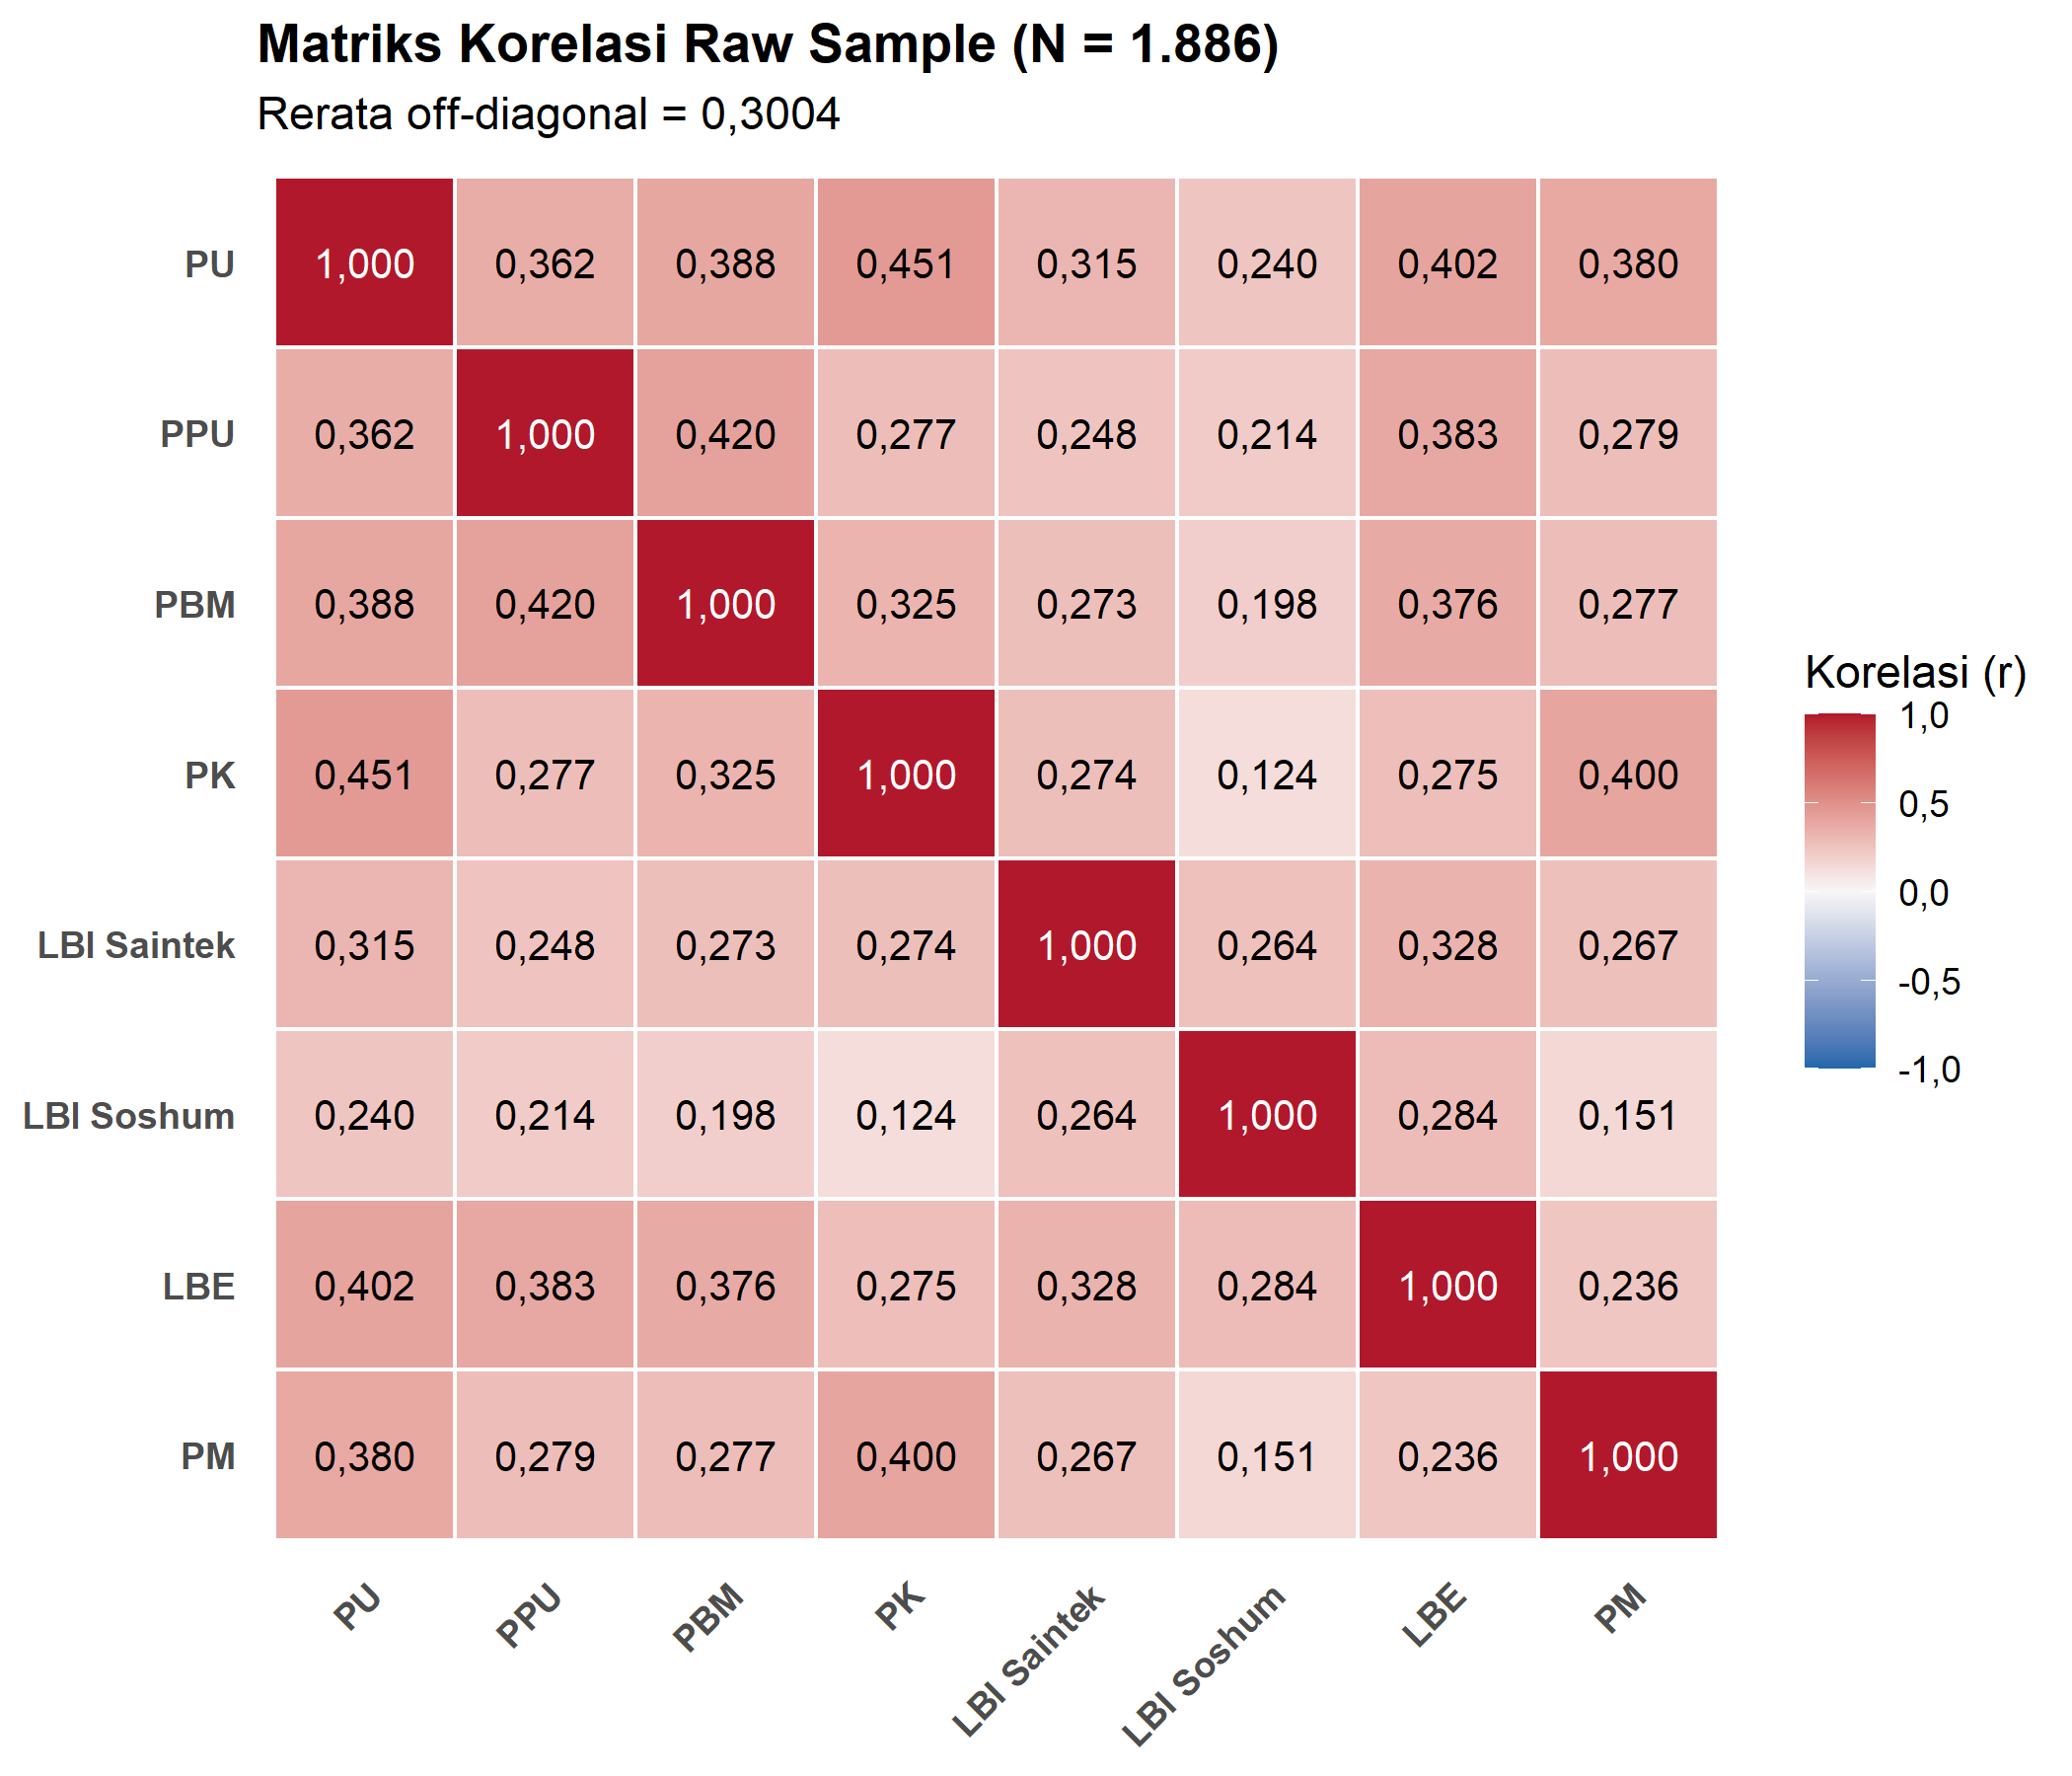
\includegraphics[width=0.65\textwidth]{../output/figures/heatmap_raw.png}
    \caption{\textit{Heatmap} Matriks Korelasi Pearson Antarsubtes (Data Sampel, $N=1.886$)}
    \label{fig:heatmap_raw}
\end{figure}

\subsection{Koreksi Kuantitatif \textit{Restriction of Range} (Thorndike Case III)}
Koreksi Thorndike Case III dengan $S_Z \approx 67,72$, hasil iterasi titik tetap, menghasilkan matriks korelasi terkoreksi dengan rerata \textit{off-diagonal} sebesar 0,425 (Tabel~\ref{tab:korelasi_terkoreksi}, Gambar~\ref{fig:heatmap_thorndike}).

\begin{table}[H]
    \centering
    \caption{Matriks Korelasi Antarsubtes Terkoreksi \textit{Restriction of Range} (Thorndike Case III)}
    \label{tab:korelasi_terkoreksi}
    \begin{spacing}{1.0}
    \resizebox{\textwidth}{!}{%
    \begin{tabular}{lcccccccc}
        \toprule
        & PU & PPU & PBM & PK & LBI Saintek & LBI Soshum & LBE & PM \\
        \midrule
        PU           & 1,000 & 0,485 & 0,514 & 0,575 & 0,447 & 0,354 & 0,527 & 0,508 \\
        PPU          & 0,485 & 1,000 & 0,523 & 0,417 & 0,374 & 0,318 & 0,494 & 0,407 \\
        PBM          & 0,514 & 0,523 & 1,000 & 0,464 & 0,401 & 0,310 & 0,495 & 0,413 \\
        PK           & 0,575 & 0,417 & 0,464 & 1,000 & 0,413 & 0,258 & 0,426 & 0,524 \\
        LBI Saintek  & 0,447 & 0,374 & 0,401 & 0,413 & 1,000 & 0,361 & 0,448 & 0,397 \\
        LBI Soshum   & 0,354 & 0,318 & 0,310 & 0,258 & 0,361 & 1,000 & 0,385 & 0,270 \\
        LBE          & 0,527 & 0,494 & 0,495 & 0,426 & 0,448 & 0,385 & 1,000 & 0,382 \\
        PM           & 0,508 & 0,407 & 0,413 & 0,524 & 0,397 & 0,270 & 0,382 & 1,000 \\
        \bottomrule
    \end{tabular}%
    }
    \end{spacing}
    \vspace{2mm}
    \begin{flushleft}
    \footnotesize\textit{Catatan.} Rerata korelasi \textit{off-diagonal} terkoreksi $\approx 0,425$.
    \end{flushleft}
\end{table}


\begin{figure}[H]
    \centering
    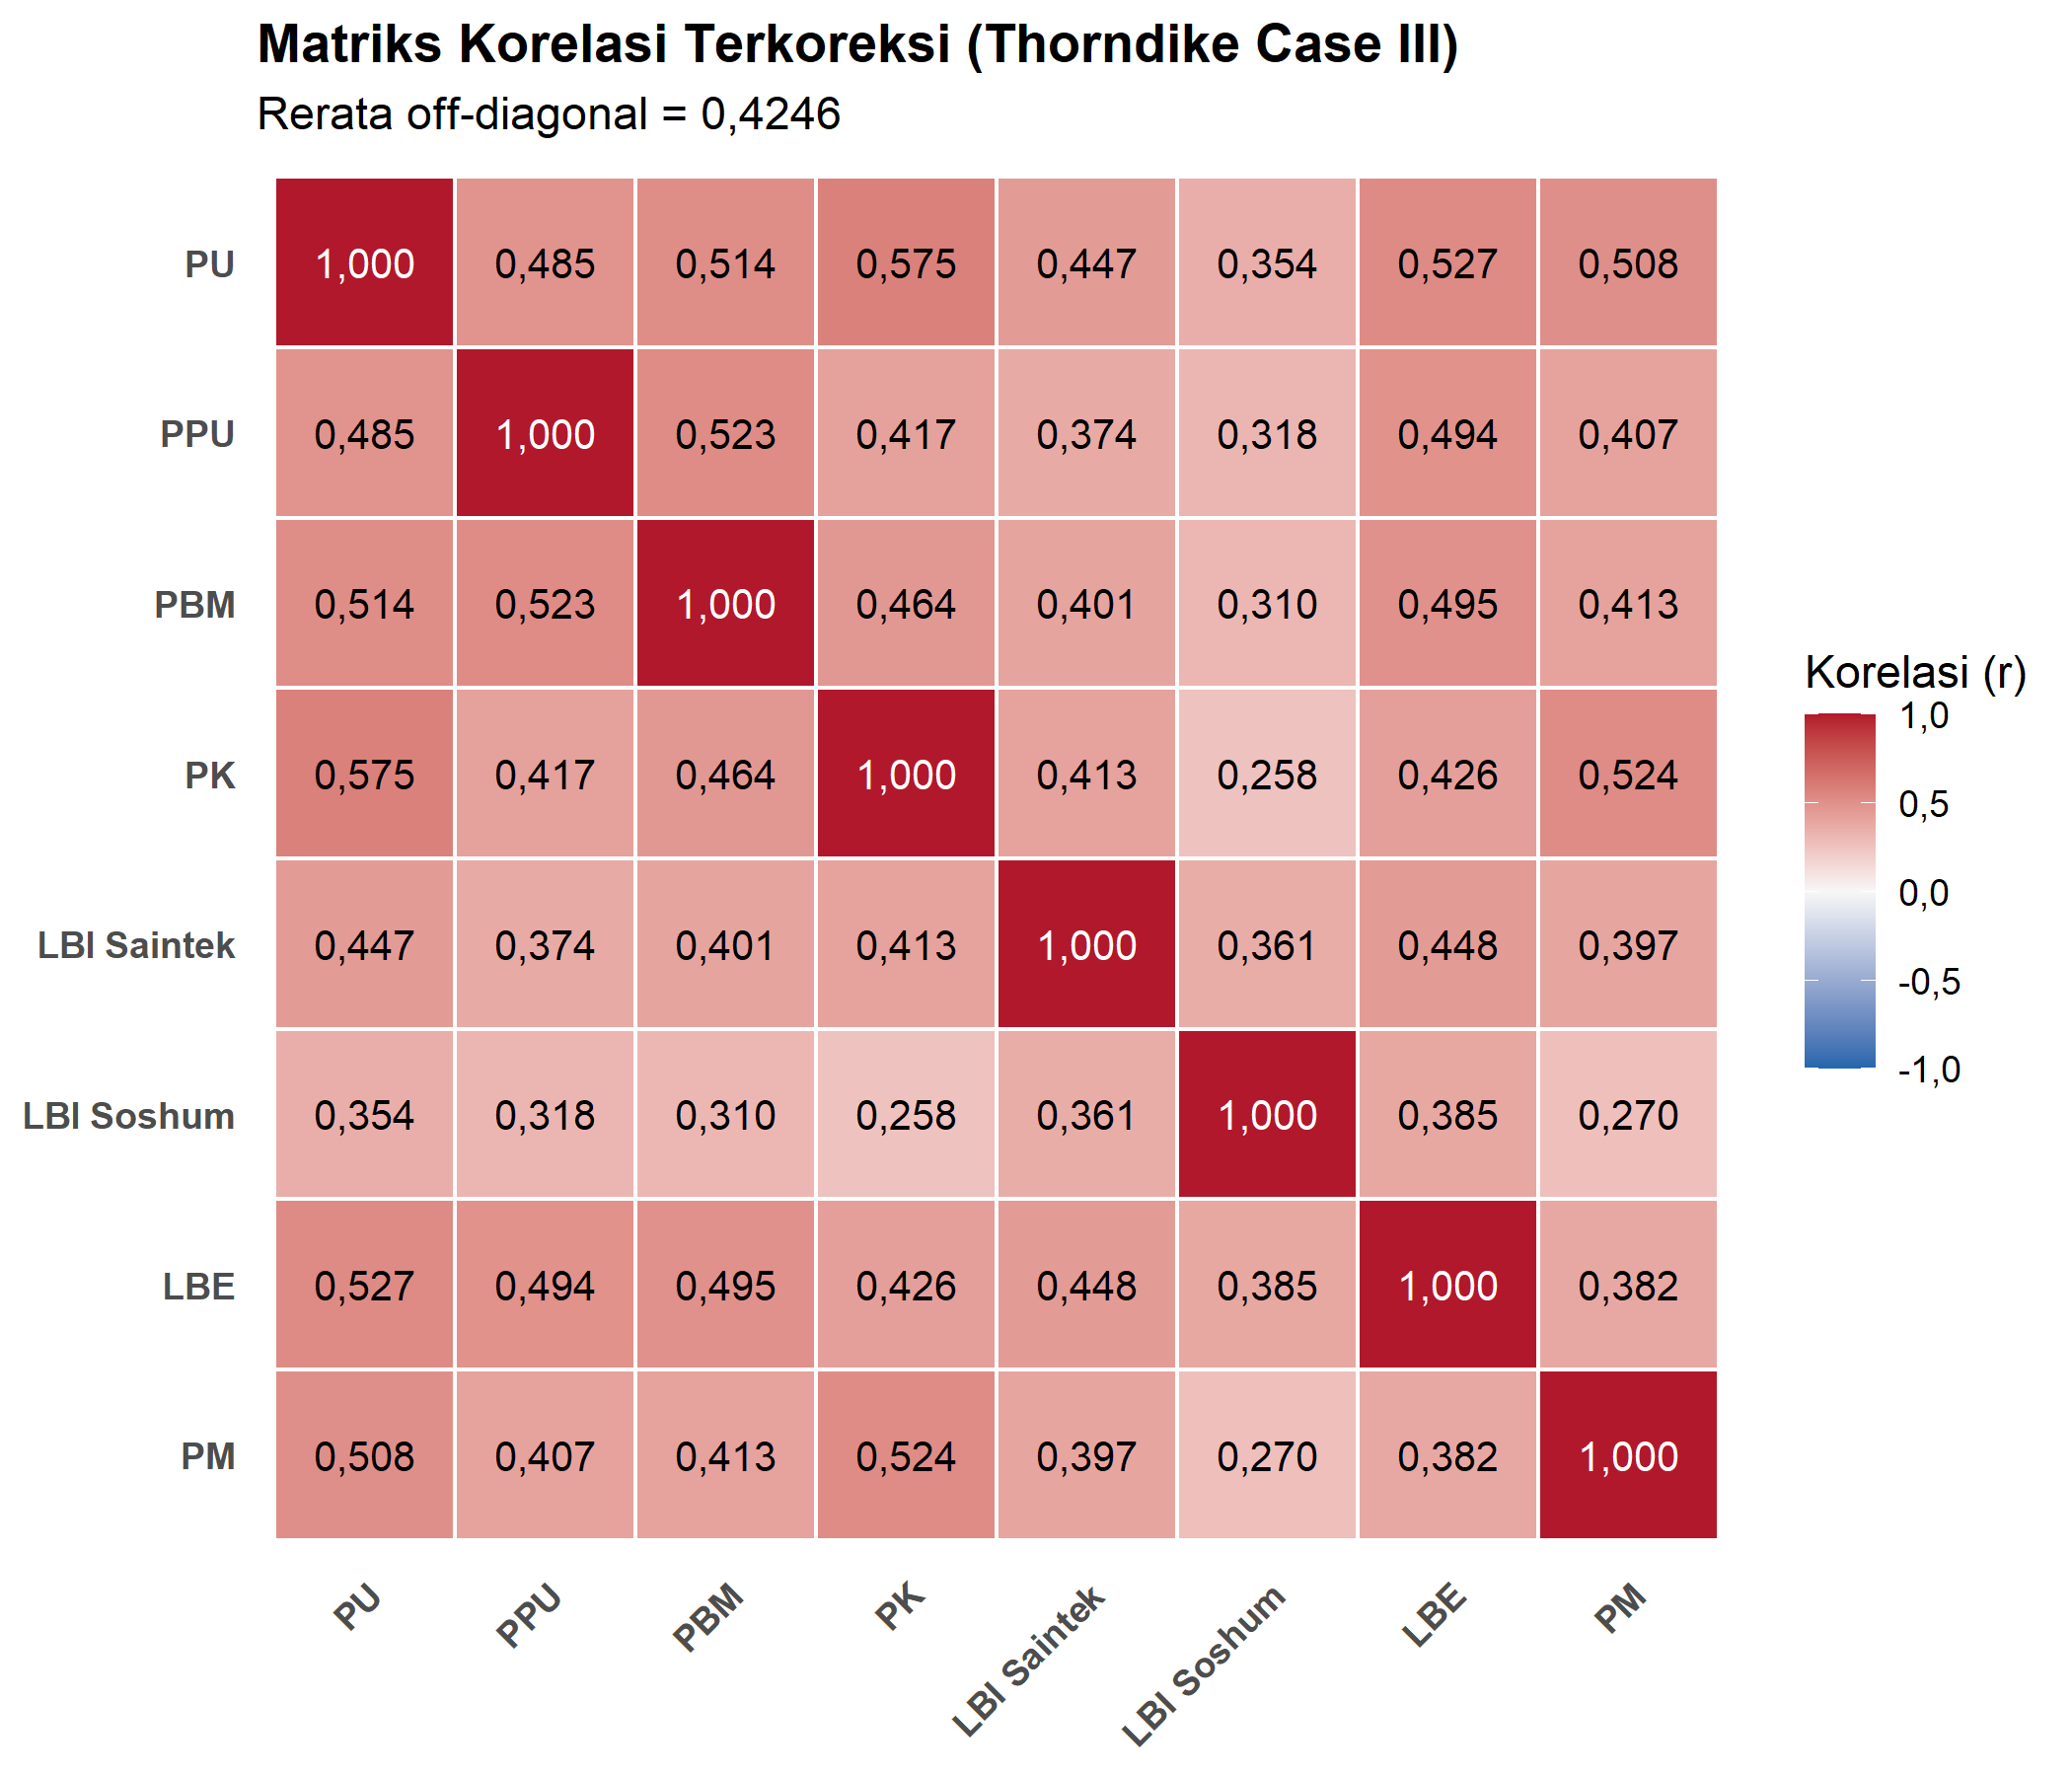
\includegraphics[width=0.65\textwidth]{../output/figures/heatmap_thorndike.png}
    \caption{\textit{Heatmap} Matriks Korelasi Antarsubtes Terkoreksi \textit{Restriction of Range} (Thorndike Case III)}
    \label{fig:heatmap_thorndike}
\end{figure}

\subsection{Analisis Faktor Eksploratori dan Konfirmatori}
Model 2 (dua faktor berkorelasi, Literasi dan Numerasi) memiliki kecocokan yang lebih baik secara signifikan dibandingkan Model 1 (\textit{g-factor} tunggal) (Tabel~\ref{tab:cfa_fit}, Gambar~\ref{fig:scree_parallel}). CFI meningkat dari $0,932$ menjadi $0,967$, RMSEA menurun dari $0,073$ menjadi $0,052$, dan uji selisih $\chi^2$ berskala Satorra--Bentler signifikan ($\Delta\chi^2(1) = 91,55$, $p < 0,001$). AIC Model 2 juga lebih rendah ($173.536,4$ berbanding $173.638,9$), sehingga Model 2 unggul pada seluruh kriteria kecocokan yang diuji.

\begin{table}[H]
    \centering
    \caption{Perbandingan Indeks Kecocokan Model 1 (\textit{g-factor} Tunggal) dan Model 2 (Dua Faktor Berkorelasi) pada CFA}
    \label{tab:cfa_fit}
    \begin{spacing}{1.0}
    \resizebox{\textwidth}{!}{%
    \begin{tabular}{lcccccccc}
        \toprule
        Model & $\chi^2_{\text{SB}}$ & $df$ & CFI & TLI & RMSEA [90\% CI] & SRMR & AIC & $\Delta\chi^2$ ($df$) \\
        \midrule
        Model 1: 1-Faktor (g-General)    & 220,17 & 20 & 0,932 & 0,904 & 0,073 [0,065; 0,082] & 0,042 & 173638,9 & - \\
        Model 2: 2-Faktor (Literasi vs Numerasi) & 117,26 & 19 & 0,967 & 0,951 & 0,052 [0,044; 0,062] & 0,031 & 173536,4 & 91,55 (1)$^{***}$ \\
        \bottomrule
    \end{tabular}%
    }
    \end{spacing}
    \vspace{2mm}
    \begin{flushleft}
    \footnotesize\textit{Catatan.} $N = 1.886$. Model 1 memuat \textit{g-factor} tunggal, sedangkan Model 2 memuat dua faktor berkorelasi (Literasi dan Numerasi). Estimator yang dipakai adalah \textit{robust maximum likelihood} (MLM). $\chi^2_{\text{SB}}$ adalah \textit{scaled chi-square} Satorra--Bentler; CFI = \textit{Comparative Fit Index}; TLI = \textit{Tucker--Lewis Index}; RMSEA = \textit{Root Mean Square Error of Approximation}; SRMR = \textit{Standardized Root Mean Square Residual}; AIC = \textit{Akaike Information Criterion}. Signifikansi $\Delta\chi^2$: $^{*}p < 0,05$; $^{**}p < 0,01$; $^{***}p < 0,001$ (dihitung dari nilai $p$ eksak).
    \end{flushleft}
\end{table}


\begin{figure}[H]
    \centering
    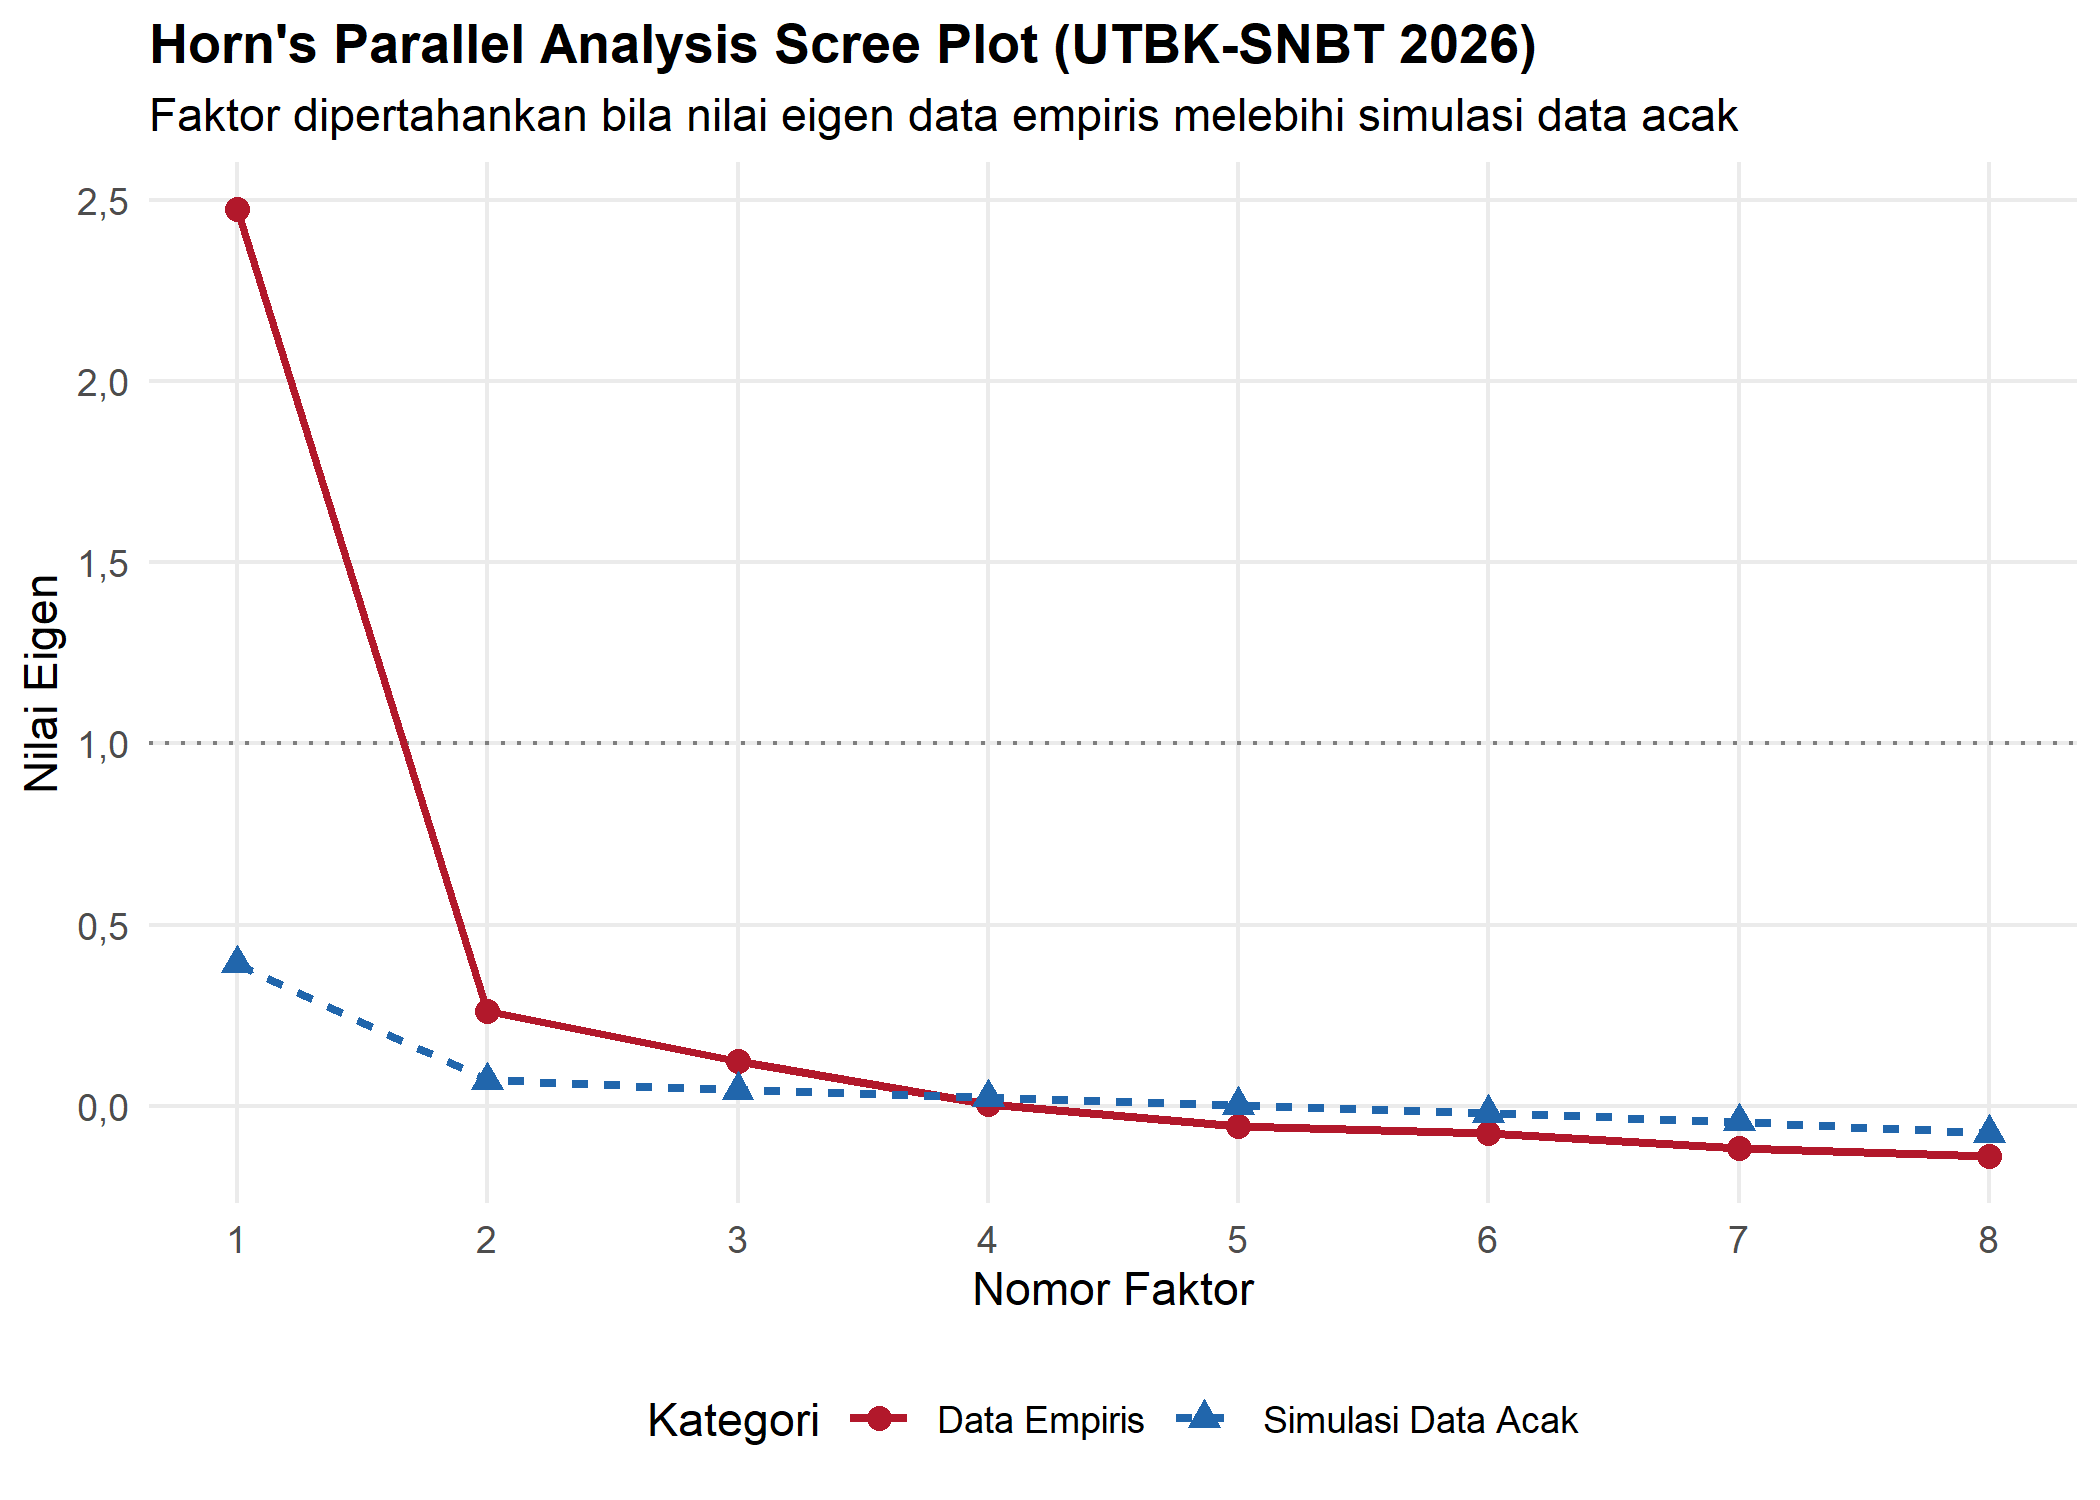
\includegraphics[width=0.65\textwidth]{../output/figures/scree_parallel_plot.png}
    \caption{\textit{Scree Plot} dan \textit{Horn's Parallel Analysis} untuk Diagnostik Retensi Faktor}
    \label{fig:scree_parallel}
\end{figure}

\textit{Parallel Analysis} berbasis faktor (Gambar~\ref{fig:scree_parallel}) menyarankan tiga faktor. Nilai eigen faktor-analitik teramati ke-1, ke-2, dan ke-3 ($2,473$; $0,261$; $0,122$) melampaui nilai eigen hasil simulasi data acak ($0,392$; $0,070$; $0,044$), sedangkan faktor ke-4 tidak ($0,006$ berbanding $0,023$). Jumlah ini berbeda dari struktur dua faktor yang ditetapkan apriori. Struktur dua faktor tetap dipertahankan karena tiga alasan: (1) pembedaan Literasi dan Numerasi bersandar pada kerangka teori yang dirumuskan sebelum analisis (lihat Tinjauan Pustaka); (2) nilai eigen faktor ketiga ($0,122$) jauh lebih kecil daripada faktor pertama ($2,473$) dan kedua ($0,261$), sehingga sumbangannya terhadap varians bersama relatif kecil; dan (3) pada sampel yang besar ($N = 1.886$), \textit{Parallel Analysis} dapat mengenali faktor kecil yang kurang bermakna secara substantif.

EFA tiga-faktor (rotasi \textit{oblimin}) menunjukkan bahwa faktor ketiga dibebani terutama oleh kedua skor LBI (LBI Soshum $0,523$; LBI Saintek $0,440$) dan sebagian oleh LBE ($0,322$). Dua faktor lainnya berisi subtes kuantitatif (PK $0,747$; PM $0,516$; PU $0,433$) dan subtes literasi umum (PPU $0,675$; PBM $0,595$; LBE $0,384$). Pola ini konsisten dengan tafsiran bahwa faktor ketiga mencerminkan varians bersama dua skor yang berasal dari satu tes LBI. Faktor itu hanya dibebani dua indikator utama, dan tafsiran ini belum diuji pada data independen. Pengaruh dependensi LBI terhadap hasil utama diperiksa pada Subbagian Sensitivitas terhadap Perlakuan Dua Skor LBI.

Sebagai pembanding, EFA dua-faktor dengan rotasi \textit{oblimin} menghasilkan kecocokan yang baik (CFI $= 0,982$; RMSEA $= 0,046$) dengan korelasi antarfaktor sebesar $0,635$, lebih rendah daripada $\phi = 0,813$ pada CFA. Selisih ini kemungkinan terkait dengan batasan nol pada \textit{cross-loading} (muatan subtes pada faktor di luar faktor utamanya) dalam model CFA. Batasan itu berpengaruh terutama pada PU, yang pada EFA membebani kedua faktor (indeks kompleksitas $1,95$, ukuran banyaknya faktor yang dimuati satu subtes). Dengan demikian, nilai $\phi$ pada CFA bergantung pada spesifikasi struktur sederhana (setiap subtes hanya memuat satu faktor).

Muatan faktor terstandarisasi pada Model 2 (Tabel~\ref{tab:factor_loadings}) menunjukkan bahwa lima subtes literasi (PPU, PBM, LBI Saintek, LBI Soshum, LBE) membebani faktor Literasi dengan muatan berkisar $0,384$--$0,629$. Tiga subtes kuantitatif (PU, PK, PM) membebani faktor Numerasi dengan muatan $0,554$--$0,736$. Seluruh muatan signifikan secara statistik ($p < 0,001$). LBI Saintek dan LBI Soshum sama-sama membebani faktor Literasi, dengan muatan LBI Soshum ($0,384$) lebih rendah daripada LBI Saintek ($0,498$). Korelasi antarfaktor laten tergolong tinggi ($\phi = 0,813$; $p < 0,001$). Meskipun Model 2 lebih unggul secara statistik, kedua faktor berbagi varians bersama yang substansial, sejalan dengan keberadaan \textit{g-factor} yang mendasari keduanya.

\begin{table}[H]
    \centering
    \caption{Muatan Faktor Terstandarisasi dan Komunalitas Subtes pada Model 2 (CFA)}
    \label{tab:factor_loadings}
    \begin{spacing}{1.0}
    \begin{tabular}{llcccc}
        \toprule
        Dimensi Laten & Subtes & $\lambda$ (Std.) & $SE$ & $z$ & $R^2$ ($h^2$) \\
        \midrule
        Literasi        & PPU          & 0,602$^{***}$ & 0,021 & 28,73 & 0,362 \\
        Literasi        & PBM          & 0,622$^{***}$ & 0,019 & 32,93 & 0,387 \\
        Literasi        & LBI Saintek  & 0,498$^{***}$ & 0,022 & 22,15 & 0,248 \\
        Literasi        & LBI Soshum   & 0,384$^{***}$ & 0,024 & 16,03 & 0,148 \\
        Literasi        & LBE          & 0,629$^{***}$ & 0,019 & 33,76 & 0,395 \\
        Numerasi        & PU           & 0,736$^{***}$ & 0,017 & 43,68 & 0,541 \\
        Numerasi        & PK           & 0,622$^{***}$ & 0,020 & 30,90 & 0,387 \\
        Numerasi        & PM           & 0,554$^{***}$ & 0,020 & 27,80 & 0,307 \\
        \bottomrule
    \end{tabular}
    \end{spacing}
    \vspace{2mm}
    \begin{flushleft}
    \footnotesize\textit{Catatan.} Bintang pada $\lambda$ menandakan signifikansi tiap muatan: $^{*}p < 0,05$; $^{**}p < 0,01$; $^{***}p < 0,001$. $SE$ = kesalahan standar; $z$ = nilai uji rasio kritis; $R^2$ ($h^2$) = proporsi varians yang dijelaskan oleh faktor laten terkait. Korelasi antarfaktor laten adalah $\phi = 0,813$$^{***}$.
    \end{flushleft}
\end{table}


\subsection{Sensitivitas terhadap Perlakuan Dua Skor LBI}
Pertama, model CFA dua-faktor diperluas dengan kovarians residual antara kedua skor LBI (Tabel~\ref{tab:sens_cfa}). Perluasan ini memperbaiki kecocokan model secara statistik ($\Delta\chi^2(1) = 17,3$, $p < 0,001$; CFI dari $0,967$ menjadi $0,973$; RMSEA dari $0,052$ menjadi $0,049$; AIC dan \textit{Bayesian Information Criterion} (BIC) menurun). Namun, korelasi residualnya kecil ($0,108$), korelasi antarfaktor hampir tidak berubah ($\phi$ dari $0,813$ menjadi $0,816$), dan muatan kedua LBI hanya bergeser sedikit (LBI Saintek dari $0,498$ menjadi $0,484$; LBI Soshum dari $0,384$ menjadi $0,365$). Dependensi antar-LBI signifikan secara statistik pada sampel sebesar ini, tetapi kecil secara praktis terhadap struktur dua-faktor.

\begin{table}[H]
    \centering
    \caption{Analisis Sensitivitas CFA Model Dua Faktor dengan dan tanpa Kovarians Residual antara LBI Saintek dan LBI Soshum}
    \label{tab:sens_cfa}
    \begin{spacing}{1.0}
    \resizebox{\textwidth}{!}{%
    \begin{tabular}{lcccccccccc}
        \toprule
        Model & $\chi^2_{\text{SB}}$ & $df$ & CFI & RMSEA & SRMR & AIC & BIC & $\phi$ & $r_{\text{resid}}$ & $\Delta\chi^2$ ($df$) \\
        \midrule
        Utama: 2-faktor & 117,3 & 19 & 0,967 & 0,052 & 0,031 & 173536 & 173631 & 0,813 & - & - \\
        2-faktor + kovarians residual LBI & 99,1 & 18 & 0,973 & 0,049 & 0,028 & 173520 & 173620 & 0,816 & 0,108 & 17,3 (1)$^{***}$ \\
        \bottomrule
    \end{tabular}%
    }
    \end{spacing}
    \vspace{2mm}
    \begin{flushleft}
    \footnotesize\textit{Catatan.} $N = 1.886$. Estimator yang dipakai adalah \textit{robust maximum likelihood} (MLM). Model utama identik dengan Model 2 pada Tabel~\ref{tab:cfa_fit}. $\phi$ = korelasi antarfaktor laten terstandar; $r_{\text{resid}}$ = korelasi residual terstandar antara LBI Saintek dan LBI Soshum. CFI = \textit{Comparative Fit Index}; RMSEA = \textit{Root Mean Square Error of Approximation}; SRMR = \textit{Standardized Root Mean Square Residual}; AIC = \textit{Akaike Information Criterion}; BIC = \textit{Bayesian Information Criterion}. Signifikansi $\Delta\chi^2$: $^{*}p < 0,05$; $^{**}p < 0,01$; $^{***}p < 0,001$ (dihitung dari nilai $p$ eksak).
    \end{flushleft}
\end{table}


Kedua, koreksi Thorndike Case III diulang dengan salah satu atau kedua skor LBI dikeluarkan dari skor komposit (Tabel~\ref{tab:sens_thorndike}). Skor komposit dihitung ulang sebagai rerata subtes yang tersisa, dan tiap subtes memakai $SD$ nasional tidak resminya sendiri. Rerata korelasi terkoreksi tetap berada pada kisaran sempit, $0,414$--$0,425$, dan $S_Z$ pada $67,43$--$68,31$, dibandingkan $\bar{R} = 0,425$ dan $S_Z = 67,72$ pada spesifikasi utama. Pembobotan ganda LBI pada skor komposit delapan subtes ($\frac{2}{8}$) tidak menggeser estimasi utama secara berarti. Rasio $SD$ tersirat terhadap $SD$ nasional tidak resmi pada keempat skenario berkisar $0,645$--$1,498$, sehingga keterbatasan homogenitas pada subbagian berikut tidak bergantung pada perlakuan LBI.

\begin{table}[H]
    \centering
    \caption{Analisis Sensitivitas Thorndike Case III terhadap Perlakuan LBI pada Skor Komposit}
    \label{tab:sens_thorndike}
    \begin{spacing}{1.0}
    \resizebox{\textwidth}{!}{%
    \begin{tabular}{lccccccc}
        \toprule
        Skenario & $k$ & $\bar{r}$ \textit{Raw Sample} & $s_Z$ Sampel & $S_Z$ Populasi & $\lambda^2$ & $\bar{R}$ Terkoreksi & Rasio $SD$ (min--maks) \\
        \midrule
        8 subtes (spesifikasi utama) & 8 & 0,300 & 53,84 & 67,72 & 0,582 & 0,425 & 0,674--1,498 \\
        7 subtes tanpa LBI Soshum & 7 & 0,330 & 57,71 & 68,03 & 0,390 & 0,424 & 0,656--1,450 \\
        7 subtes tanpa LBI Saintek & 7 & 0,307 & 55,47 & 67,43 & 0,478 & 0,414 & 0,666--1,475 \\
        6 subtes tanpa kedua LBI & 6 & 0,349 & 60,43 & 68,31 & 0,278 & 0,421 & 0,645--1,419 \\
        \bottomrule
    \end{tabular}%
    }
    \end{spacing}
    \vspace{2mm}
    \begin{flushleft}
    \footnotesize\textit{Catatan.} Skor komposit adalah rerata $k$ subtes yang dipakai, dan tiap subtes memakai $SD$ nasional tidak resminya sendiri. $\bar{r}$ adalah rerata korelasi \textit{raw sample}, dan $\bar{R}$ adalah rerata korelasi terkoreksi \textit{restriction of range}. $\lambda^2$ adalah multiplikator seleksi ($\frac{S_Z^2}{s_Z^2} - 1$). Rasio adalah $SD$ tersirat populasi terhadap $SD$ nasional tidak resmi (lihat Tabel~\ref{tab:diagnostik}). Rerata kedua skor LBI tidak dipakai karena $SD$ nasionalnya tidak tersedia.
    \end{flushleft}
\end{table}


\subsection{Evaluasi Homogenitas Struktur Korelasi Antarsubtes}
Koreksi Thorndike Case III mengasumsikan struktur korelasi yang relatif seragam antarpasangan subtes untuk menurunkan $SD$ skor komposit populasi tersirat. Kewajaran asumsi itu diuji dengan menghitung $SD$ populasi tersirat tiap subtes menggunakan korelasi tiap subtes terhadap skor komposit ($r_{iZ}$, korelasi item-total; Tabel~\ref{tab:diagnostik}), lalu membandingkannya dengan $SD$ nasional tidak resminya.

\begin{table}[H]
    \centering
    \caption{Diagnostik Deviasi $SD$ Tersirat dari Korelasi Item-Total terhadap $SD$ Nasional per Subtes}
    \label{tab:diagnostik}
    \begin{spacing}{1.0}
    \begin{tabular}{lccccc}
        \toprule
        Subtes & $SD$ Sampel & $r_{iz}$ & $SD$ Tersirat Populasi & $SD$ Nasional & Rasio \\
        \midrule
        PU              & 76,85 & 0,706 & 87,27 & 71,52 & 1,220 \\
        PPU             & 61,50 & 0,590 & 67,45 & 100,00 & 0,674 \\
        PBM             & 76,62 & 0,631 & 85,03 & 100,00 & 0,850 \\
        PK              & 131,90 & 0,705 & 149,75 & 100,00 & 1,498 \\
        LBI Saintek     & 82,31 & 0,586 & 90,15 & 100,00 & 0,902 \\
        LBI Soshum      & 70,11 & 0,452 & 74,15 & 100,00 & 0,742 \\
        LBE             & 86,50 & 0,642 & 96,32 & 100,00 & 0,963 \\
        PM              & 100,01 & 0,634 & 111,10 & 100,00 & 1,111 \\
        \bottomrule
    \end{tabular}
    \end{spacing}
    \vspace{2mm}
    \begin{flushleft}
    \footnotesize\textit{Catatan.} Rasio = $SD$ tersirat populasi $\div$ $SD$ nasional. Rasio yang menyimpang jauh dari 1 mengindikasikan pelanggaran asumsi korelasi seragam yang disyaratkan koreksi Case III untuk subtes itu.
    \end{flushleft}
\end{table}


Rasio bervariasi cukup lebar (0,674--1,498), dan variasi ini mengindikasikan bahwa asumsi homogenitas korelasi tidak terpenuhi secara seragam pada seluruh subtes. Deviasi terbesar teramati pada PK (rasio $1,498$), yang konsisten dengan nilai ekstrem pada subtes itu (lihat Subbagian Evaluasi Asumsi Distribusi). Deviasi besar juga teramati pada PPU (rasio $0,674$) dan LBI Soshum (rasio $0,742$), yang keduanya memiliki $SD$ tersirat jauh di bawah $SD$ nasional tidak resmi. Sebaliknya, PU, PBM, LBI Saintek, LBE, dan PM memiliki rasio yang relatif mendekati satu ($0,850$--$1,220$), sehingga asumsi Case III lebih sesuai untuk subtes-subtes itu. Pola ini mengindikasikan bahwa $\bar{R} \approx 0,425$ paling tepat ditafsirkan sebagai rerata populasi yang menyamaratakan heterogenitas riil antarsubtes. Keterbatasan ini dicatat lebih lanjut pada Bagian Keterbatasan Penelitian.

\subsection{Ketidakpastian Estimasi dari \textit{Bootstrap} dan Sensitivitas terhadap $SD$ Nasional}
Dari 2.000 replikasi \textit{bootstrap}, seluruhnya konvergen (Tabel~\ref{tab:bootstrap}). Interval persentil 95\% untuk $S_Z$ adalah $[66,6; 68,8]$ di sekitar estimasi $67,7$ ($SE = 0,55$), untuk $\lambda^2$ adalah $[0,479; 0,700]$, dan untuk $\bar{R}$ adalah $[0,407; 0,442]$ ($SE = 0,009$). Pada skala skor komposit, interval $S_Z$ itu hanya menggeser skor sekitar tiga poin atau kurang pada $M \pm 3\,SD$. Skor komposit pada $M + 2\,SD$ sekitar $635$ (interval $633$--$638$), pada $M + 3\,SD$ sekitar $703$ ($700$--$706$), dan pada $M - 3\,SD$ sekitar $297$ ($294$--$300$).

\begin{table}[H]
    \centering
    \caption{Interval \textit{Bootstrap} 95\% untuk Estimasi Utama Thorndike Case III (Delapan Subtes)}
    \label{tab:bootstrap}
    \begin{spacing}{1.0}
    \begin{tabular}{lcccc}
        \toprule
        Statistik & Estimasi & Rerata \textit{Bootstrap} & $SE$ \textit{Bootstrap} & Interval Persentil 95\% \\
        \midrule
        $S_Z$ populasi & 67,72 & 67,73 & 0,55 & [66,63; 68,79] \\
        $\lambda^2$ & 0,582 & 0,586 & 0,058 & [0,479; 0,700] \\
        $\bar{R}$ terkoreksi & 0,425 & 0,425 & 0,009 & [0,407; 0,442] \\
        \bottomrule
    \end{tabular}
    \end{spacing}
    \vspace{2mm}
    \begin{flushleft}
    \footnotesize\textit{Catatan.} Interval dihitung dengan \textit{bootstrap} nonparametrik (penarikan ulang entri sampel teramati) sebanyak 2.000 replikasi, 2.000 di antaranya konvergen. Interval hanya menangkap ketidakpastian pengambilan sampel dan mengandaikan $SD$ nasional serta spesifikasi Case III benar (lihat Tabel~\ref{tab:sens_sd}).
    \end{flushleft}
\end{table}


Estimasi jauh lebih peka terhadap perubahan $SD$ nasional daripada terhadap pengambilan sampel (Tabel~\ref{tab:sens_sd}). Perubahan seluruh $SD$ sebesar $\pm 5\%$ menggeser $\bar{R}$ menjadi $0,367$ dan $0,475$ ($S_Z$ $60,9$ dan $74,2$), dan perubahan $\pm 10\%$ menggesernya menjadi $0,300$ dan $0,519$ ($S_Z$ $53,8$ dan $80,5$). Pada pengali $0,90$, $\lambda^2$ mendekati nol ($-0,002$) dan $S_Z$ ($53,79$) hampir sama dengan $s_Z$ ($53,84$), sehingga koreksi Case III praktis tidak mengubah korelasi sampel ($\bar{R} = 0,300$). Pada skenario ini, skor komposit sampel tidak menunjukkan \textit{restriction of range} terhadap populasi yang diasumsikan. Mengganti $SD_{\text{PU}}$ dari $71,52$ menjadi $100$ menaikkan $\bar{R}$ menjadi $0,466$ ($S_Z = 73,0$). Rasio $SD$ tersirat terhadap $SD$ nasional tetap bervariasi antarsubtes pada semua skenario (minimum $0,669$--$0,699$; maksimum $1,46$--$1,57$), sehingga temuan heterogenitas pada Subbagian Evaluasi Homogenitas Struktur Korelasi Antarsubtes tidak bergantung pada skala $SD$ yang diasumsikan.

Hasil ini menunjukkan bahwa $\bar{R} \approx 0,425$ dan $S_Z \approx 67,72$ bersifat kondisional terhadap parameter nasional yang belum terverifikasi, dan bahwa interval \textit{bootstrap} hanya mencerminkan sebagian ketidakpastian (lihat Keterbatasan Penelitian).

\begin{table}[H]
    \centering
    \caption{Sensitivitas Estimasi Thorndike Case III terhadap Simpangan Baku Nasional Tidak Resmi}
    \label{tab:sens_sd}
    \begin{spacing}{1.0}
    \resizebox{\textwidth}{!}{%
    \begin{tabular}{lcccc}
        \toprule
        Skenario & $S_Z$ Populasi & $\lambda^2$ & $\bar{R}$ Terkoreksi & Rasio $SD$ (min--maks) \\
        \midrule
        $SD$ nasional tanpa penyesuaian (utama) & 67,72 & 0,582 & 0,425 & 0,674--1,498 \\
        Semua $SD$ $\times$ 0,90 & 53,79 & -0,002 & 0,300 & 0,683--1,465 \\
        Semua $SD$ $\times$ 0,95 & 60,93 & 0,281 & 0,367 & 0,678--1,482 \\
        Semua $SD$ $\times$ 1,05 & 74,22 & 0,900 & 0,475 & 0,671--1,511 \\
        Semua $SD$ $\times$ 1,10 & 80,52 & 1,236 & 0,519 & 0,669--1,523 \\
        $SD_{\text{PU}} = 100$ ($SD$ lain tetap) & 72,98 & 0,837 & 0,466 & 0,699--1,570 \\
        \bottomrule
    \end{tabular}%
    }
    \end{spacing}
    \vspace{2mm}
    \begin{flushleft}
    \footnotesize\textit{Catatan.} Sampel dan korelasi tidak diubah; hanya $SD$ nasional tidak resmi yang dikalikan faktor tertentu atau (pada baris terakhir) diganti. Rasio = $SD$ tersirat populasi terhadap $SD$ nasional pada skenario yang sama.
    \end{flushleft}
\end{table}


\subsection{Sensitivitas terhadap Korelasi yang Bergantung pada Tingkat Skor}
Data ini tidak dapat memisahkan \textit{restriction of range} dari diferensiasi kemampuan (lihat Pembahasan), sehingga dampak SLODR hanya dapat diperiksa melalui skenario simulasi. Skenario $b = 0,02$ menghasilkan korelasi bersyarat $0,446$ pada $g = -1$ dan $0,395$ pada $g = +1$, sedangkan skenario $b = 0,04$ menghasilkan $0,479$ dan $0,375$.

Pada bagian pertama simulasi (Tabel~\ref{tab:slodr_ekor}), $SD$ skor komposit tetap $67,72$ pada tiap $b$. Penurunan korelasi pada skor tinggi menipiskan ekor atas dan menebalkan ekor bawah, sehingga kemiringan ke kanan yang berasal dari marginal berkurang. \textit{Skewness} skor komposit turun dari $0,418$ ($b = 0$) menjadi $0,304$ ($b = 0,02$) dan $0,195$ ($b = 0,04$). Peluang melampaui $M + 2\,S_Z$ turun dari $3,33\%$ menjadi $3,02\%$ dan $2,72\%$ (normal $2,28\%$), dan peluang melampaui $M + 3\,S_Z$ turun dari $0,379\%$ menjadi $0,257\%$ dan $0,161\%$ (normal $0,135\%$). Skor komposit pada persentil normal ke-99,9 turun dari $730$ menjadi $718$ dan $707$ (normal $703$), sedangkan pada persentil normal ke-97,7 turun dari $649$ menjadi $645$ dan $641$ (normal $635$). Di ekor bawah, peluang berada di bawah $M - 2\,S_Z$ naik dari $0,81\%$ menjadi $1,11\%$ dan $1,43\%$, masih di bawah $2,28\%$ pada normal. Perubahan di sekitar $\pm 1\,SD$ kecil (selisih skor kurang dari $1,6$ poin pada semua skenario).

\begin{table}[H]
    \centering
    \caption{Dampak Skenario SLODR terhadap Ekor Distribusi Skor Komposit (Marginal Johnson SB, \textit{Copula} Gaussian)}
    \label{tab:slodr_ekor}
    \begin{spacing}{1.0}
    \resizebox{\textwidth}{!}{%
    \begin{tabular}{lcccccc}
        \toprule
        & Normal & \multicolumn{5}{c}{Kemiringan SLODR $b$} \\
        \cmidrule(lr){3-7}
        & & 0,00 & 0,01 & 0,02 & 0,03 & 0,04 \\
        \midrule
        Skewness komposit & $0{,}000$ & 0,419 & 0,361 & 0,304 & 0,249 & 0,195 \\
        \midrule
        \multicolumn{7}{l}{\textit{Peluang ekor (\%)}} \\
        $M - 3\,S_Z$ & 0,135 & $<0{,}001$ & $<0{,}001$ & $<0{,}001$ & 0,001 & 0,003 \\
        $M - 2\,S_Z$ & 2,275 & 0,812 & 0,965 & 1,110 & 1,273 & 1,432 \\
        $M + 2\,S_Z$ & 2,275 & 3,327 & 3,180 & 3,026 & 2,881 & 2,716 \\
        $M + 3\,S_Z$ & 0,135 & 0,380 & 0,318 & 0,257 & 0,206 & 0,161 \\
        \midrule
        \multicolumn{7}{l}{\textit{Skor komposit pada persentil normal}} \\
        $M - 3\,S_Z$ & 296,9 & 341,8 & 338,4 & 335,3 & 332,1 & 328,9 \\
        $M - 2\,S_Z$ & 364,6 & 381,7 & 379,8 & 377,8 & 375,9 & 374,1 \\
        $M + 2\,S_Z$ & 635,4 & 648,9 & 647,0 & 644,8 & 642,6 & 640,7 \\
        $M + 3\,S_Z$ & 703,1 & 730,3 & 724,4 & 718,4 & 712,3 & 707,1 \\
        \bottomrule
    \end{tabular}%
    }
    \end{spacing}
    \vspace{2mm}
    \begin{flushleft}
    \footnotesize\textit{Catatan.} SLODR adalah \textit{Spearman's Law of Diminishing Returns}, yaitu gagasan bahwa korelasi antartes menurun pada kemampuan tinggi. Muatan \textit{g-factor} ditetapkan sebagai $m(g) = m_0 - b\,g$ dengan $g \sim N(0,1)$; $b = 0$ berarti korelasi konstan. $m_0$ dikalibrasi pada tiap $b$ sehingga $SD$ komposit $= S_Z = 67,72$; skor komposit dipusatkan ke $500$. Peluang ekor mengacu pada sisi bawah untuk $k<0$ dan sisi atas untuk $k>0$. Korelasi bersyarat pada $g=-1$, $+1$, dan $+2$ masing-masing $0,446$, $0,394$, dan $0,370$ pada $b = 0,02$.
    \end{flushleft}
\end{table}


Pada bagian kedua simulasi (Tabel~\ref{tab:slodr_case3}), sampel simulasi disamakan dengan sampel teramati (rerata skor komposit $657,8$; $SD$ $53,8$; rerata korelasi \textit{raw sample} $0,300$), lalu koreksi dijalankan dan dibandingkan dengan nilai sebenarnya pada populasi simulasi. Karena sampel yang disimulasikan sama pada semua $b$, taksiran Case III identik ($\bar{R} = 0,437$; $S_Z = 68,7$), sedangkan nilai sebenarnya berubah. Pada $b = 0$ koreksi memulihkan nilai sebenarnya dengan baik (bias $\bar{R}$ $-0,002$; bias $S_Z$ $-0,2$), sehingga prosedur dapat dipercaya bila asumsinya terpenuhi. Pada $b = 0,02$, $\bar{R}$ sebenarnya $0,499$ (bias $-0,061$) dan $S_Z$ sebenarnya $72,3$ (bias $-3,6$). Pada $b = 0,04$, nilai itu masing-masing $0,561$ (bias $-0,123$) dan $75,7$ (bias $-7,0$). Dalam model ini, koreksi Case III menaksir rendah korelasi dan $SD$ populasi bila SLODR berlaku, dan taksiran makin rendah pada $b$ yang makin besar. Taksiran simulasi pada $b = 0$ ($0,437$) sedikit berbeda dari estimasi utama ($0,425$) karena populasi simulasi bersifat Gaussian, dan perbedaan ini kecil dibandingkan dengan bias pada $b > 0$.

\begin{table}[H]
    \centering
    \caption{Kinerja Koreksi Thorndike Case III pada Populasi Simulasi dengan Korelasi yang Menurun pada Skor Tinggi (SLODR)}
    \label{tab:slodr_case3}
    \begin{spacing}{1.0}
    \resizebox{\textwidth}{!}{%
    \begin{tabular}{ccccccccc}
        \toprule
        & \multicolumn{2}{c}{Korelasi Bersyarat} & \multicolumn{3}{c}{$\bar{R}$} & \multicolumn{3}{c}{$S_Z$} \\
        \cmidrule(lr){2-3} \cmidrule(lr){4-6} \cmidrule(lr){7-9}
        $b$ & $g=-1$ & $g=+1$ & Benar & Case III & Bias & Benar & Case III & Bias \\
        \midrule
        0,00 & 0,440 & 0,440 & 0,440 & 0,437 & -0,002 & 68,9 & 68,7 & -0,2 \\
        0,02 & 0,527 & 0,470 & 0,499 & 0,437 & -0,061 & 72,3 & 68,7 & -3,6 \\
        0,04 & 0,620 & 0,501 & 0,561 & 0,437 & -0,123 & 75,7 & 68,7 & -7,0 \\
        \bottomrule
    \end{tabular}%
    }
    \end{spacing}
    \vspace{2mm}
    \begin{flushleft}
    \footnotesize\textit{Catatan.} SLODR adalah \textit{Spearman's Law of Diminishing Returns}. Populasi Gaussian dengan $SD$ nasional tidak resmi dan muatan $m(g) = m_0 - b\,g$; sampel terseleksi lewat skor komposit (probabilitas seleksi logistik) dikalibrasi agar sama dengan sampel teramati (rerata skor komposit 657,8, $SD$ 53,8, rerata korelasi \textit{raw sample} 0,300). Karena sampel sama pada semua $b$, taksiran Case III identik; kolom Benar adalah nilai pada populasi simulasi. Bias = Case III $-$ Benar.
    \end{flushleft}
\end{table}


Model satu faktor dengan muatan linear terhadap $g$ hanyalah satu bentuk SLODR di antara banyak kemungkinan, dan data ini tidak dapat menunjukkan apakah $b$ sebesar itu, lebih kecil, atau nol.

\subsection{Tren Estimasi Korelasi Sepanjang Proses Pengumpulan Data}
Rerata korelasi \textit{off-diagonal} tidak konstan selama pengumpulan data. Estimasi berfluktuasi, lalu melandai (\textit{plateau}) seiring penambahan sampel (Tabel~\ref{tab:saturasi_tahap}).

\begin{table}[H]
    \centering
    \caption{Rerata Korelasi \textit{Off-Diagonal} Antarsubtes secara Kumulatif Seiring Bertambahnya Tahap Pengumpulan Data}
    \label{tab:saturasi_tahap}
    \begin{spacing}{1.0}
    \resizebox{\textwidth}{!}{%
    \begin{tabular}{cllcc}
        \toprule
        Tahap & Nama Tahap & Kategori & $N$ Kumulatif & $\bar{r}$ \textit{off-diagonal} \\
        \midrule
        1 & Utas Tunggal \& DM Pribadi     & Campuran        & 216 & 0,297 \\
        2 & Utas Khusus Unpad              & PTN Khusus      & 249 & 0,300 \\
        3 & Utas Khusus PENS               & PTN Khusus      & 255 & 0,298 \\
        4 & Utas Khusus Unsoed             & PTN Khusus      & 289 & 0,298 \\
        5 & Utas Khusus Unesa              & PTN Khusus      & 300 & 0,293 \\
        6 & Utas Khusus Unnes              & PTN Khusus      & 320 & 0,286 \\
        7 & Utas Khusus ITS                & PTN Khusus      & 416 & 0,345 \\
        8 & Utas Khusus Undip              & PTN Khusus      & 567 & 0,316 \\
        9 & Utas Khusus IPB                & PTN Khusus      & 613 & 0,304 \\
        10 & Utas Khusus UNS                & PTN Khusus      & 675 & 0,294 \\
        11 & Utas Khusus UB                 & PTN Khusus      & 816 & 0,269 \\
        12 & Utas Khusus UPI                & PTN Khusus      & 847 & 0,267 \\
        13 & Utas Khusus UGM                & PTN Khusus      & 992 & 0,280 \\
        14 & Utas Khusus Unair              & PTN Khusus      & 1.095 & 0,270 \\
        15 & Utas Khusus PNJ                & PTN Khusus      & 1.107 & 0,269 \\
        16 & Utas Khusus UI                 & PTN Khusus      & 1.319 & 0,286 \\
        17 & Utas Khusus ITB                & PTN Khusus      & 1.459 & 0,305 \\
        18 & Utas Terbuka Inklusif (@sbmptnfess) & Inklusif        & 1.709 & 0,309 \\
        19 & Akun Publik @utbkcak           & Inklusif        & 1.886 & 0,300 \\
        \bottomrule
    \end{tabular}%
    }
    \end{spacing}
    \vspace{2mm}
    \begin{flushleft}
    \footnotesize\textit{Catatan.} $N$ kumulatif adalah jumlah entri dari Tahap 1 sampai tahap terkait (tahap disusun berurutan sesuai kronologi pengumpulan). Nilai $\bar{r}$ \textit{off-diagonal}, yaitu rerata korelasi di luar diagonal matriks korelasi \textit{raw sample}, dihitung ulang dari entri kumulatif itu.
    \end{flushleft}
\end{table}


Pada 17 tahap awal, yaitu utas khusus per-PTN (Tahap 1 hingga 17, $N = 216$ hingga $N = 1.459$), estimasi korelasi kumulatif berfluktuasi antara $0,267$ pada Tahap 12 (Universitas Pendidikan Indonesia, UPI) dan $0,345$ pada Tahap 7 (Institut Teknologi Sepuluh Nopember, ITS). Fluktuasi ini mencerminkan perbedaan varians skor pada tiap klaster PTN yang masuk secara berurutan. Korelasi melonjak tajam setelah data ITS, yang memiliki sebaran skor kuantitatif tinggi, ditambahkan (Tahap 7). Korelasi kemudian menurun bertahap seiring masuknya klaster PTN dengan sebaran skor lokal yang relatif lebih homogen, yaitu UB, UPI, UGM, Universitas Airlangga (Unair), dan Politeknik Negeri Jakarta (PNJ) pada Tahap 11--15. Setelah itu, korelasi meningkat kembali menjelang penambahan data Universitas Indonesia (Tahap 16, $r = 0,286$) dan Institut Teknologi Bandung (Tahap 17, $r = 0,305$).

Sebaliknya, Tahap 18 (utas terbuka inklusif @sbmptnfess, $N = 1.709$) dan Tahap 19 (akun publik @utbkcak, $N = 1.886$) hanya mengubah estimasi secara marjinal ($0,300$--$0,309$). Kedua tahap itu secara desain ditujukan untuk menjaring variasi skor yang lebih luas tanpa syarat kelulusan. Hasil ini mengindikasikan bahwa sampel telah mencapai batas keterwakilan maksimal (\textit{saturation plateau}) yang dapat diperoleh dari karakteristik audiens platform terkait.

\subsection{Matriks Translasi Persentil Standar}
Sebagai aplikasi praktis dari parameter nasional tidak resmi dan estimasi korelasi, Tabel~\ref{tab:ranking_subtes} menyajikan translasi tujuh titik \textit{benchmark} persentil standar ($M \pm k\,SD$, $k = 0, 1, 2, 3$) ke skor mentah tiap subtes, dengan $SD$ nasional tidak resmi per subtes ($SD_{\text{PU}} = 71,52$; $SD_{\text{subtes lain}} = 100$). Persentil dihitung langsung dari distribusi normal baku terhadap parameter populasi ($N_{\text{nasional}} = 846.518$ peserta hadir), sehingga nilai persentil pada tiap baris identik lintas subtes secara desain. Hanya skor mentah yang berbeda, mengikuti perbedaan $SD$ nasional antarsubtes.

\begin{table}[H]
    \centering
    \caption{Matriks Translasi Persentil Standar ke Skor Mentah per Subtes ($M = 500$, $SD$ Nasional Tidak Resmi per Subtes)}
    \label{tab:ranking_subtes}
    \begin{spacing}{1.0}
    \resizebox{\textwidth}{!}{%
    \begin{tabular}{lcccccccccc}
        \toprule
        Titik \textit{Benchmark} & Persentil (\%) & Peringkat Nasional & PU & PPU & PBM & PK & LBI Saintek & LBI Soshum & LBE & PM \\
        \midrule
        M - 3 SD   & 99,87 & 845.375 & 285,44 & 200,00 & 200,00 & 200,00 & 200,00 & 200,00 & 200,00 & 200,00 \\
        M - 2 SD   & 97,72 & 827.260 & 356,96 & 300,00 & 300,00 & 300,00 & 300,00 & 300,00 & 300,00 & 300,00 \\
        M - 1 SD   & 84,13 & 712.213 & 428,48 & 400,00 & 400,00 & 400,00 & 400,00 & 400,00 & 400,00 & 400,00 \\
        M          & 50,00 & 423.259 & 500,00 & 500,00 & 500,00 & 500,00 & 500,00 & 500,00 & 500,00 & 500,00 \\
        M + 1 SD   & 15,87 & 134.305 & 571,52 & 600,00 & 600,00 & 600,00 & 600,00 & 600,00 & 600,00 & 600,00 \\
        M + 2 SD   & 2,28 & 19.258 & 643,04 & 700,00 & 700,00 & 700,00 & 700,00 & 700,00 & 700,00 & 700,00 \\
        M + 3 SD   & 0,13 & 1.143 & 714,56 & 800,00 & 800,00 & 800,00 & 800,00 & 800,00 & 800,00 & 800,00 \\
        \bottomrule
    \end{tabular}%
    }
    \end{spacing}
    \vspace{2mm}
    \begin{flushleft}
    \footnotesize\textit{Catatan.} Persentil (\textit{top \%}) identik lintas subtes pada baris yang sama secara desain. Hanya skor mentah yang berbeda antarsubtes karena perbedaan $SD$ nasional. Peringkat nasional dihitung dari jumlah peserta hadir, $N_{\text{nasional}} = 846.518$.
    \end{flushleft}
\end{table}


Tabel~\ref{tab:ranking_komposit} memperluas translasi itu ke skor komposit dengan membandingkan tujuh skenario asumsi korelasi antarsubtes. Skenario itu disusun simetris di sekitar estimasi Thorndike Case III, yakni tiga skenario di bawahnya dan tiga di atasnya. Ketujuh skenario adalah korelasi \textit{raw sample} ($r \approx 0,300$), estimasi terkoreksi Thorndike Case III ($R \approx 0,425$; $S_Z \approx 67,72$), dan lima titik hipotetis pada rentang $r = 0,350$--$0,550$. Kelima titik hipotetis berfungsi sebagai analisis sensitivitas. Perbedaan asumsi korelasi berdampak besar pada skor komposit di persentil ekstrem. Pada titik $M + 2\,SD$, misalnya, skor komposit berkisar dari $620,25$ (korelasi \textit{raw sample}) hingga $650,25$ (skenario $r = 0,550$), dengan estimasi Thorndike Case III pada $635,43$. Selisih hingga 30 poin itu murni berasal dari perbedaan asumsi struktur korelasi. Pola ini menunjukkan bahwa penerjemahan skor komposit ke persentil nasional sensitif terhadap ketepatan estimasi korelasi antarsubtes yang digunakan.

\begin{table}[H]
    \centering
    \caption{Matriks Translasi Persentil Standar ke Skor Komposit Lintas Skenario Korelasi Antarsubtes ($M = 500$)}
    \label{tab:ranking_komposit}
    \begin{spacing}{1.0}
    \resizebox{\textwidth}{!}{%
    \begin{tabular}{lccccccccc}
        \toprule
        Titik \textit{Benchmark} & Persentil (\%) & Peringkat Nasional & Raw Sample & r = 0.350 & r = 0.400 & Thorndike Case III & r = 0.450 & r = 0.500 & r = 0.550 \\
        \midrule
        M - 3 SD   & 99,87 & 845.375 & 319,63 & 309,83 & 300,45 & 296,85 & 291,49 & 282,90 & 274,63 \\
        M - 2 SD   & 97,72 & 827.260 & 379,75 & 373,22 & 366,97 & 364,57 & 360,99 & 355,26 & 349,75 \\
        M - 1 SD   & 84,13 & 712.213 & 439,88 & 436,61 & 433,48 & 432,28 & 430,50 & 427,63 & 424,88 \\
        M          & 50,00 & 423.259 & 500,00 & 500,00 & 500,00 & 500,00 & 500,00 & 500,00 & 500,00 \\
        M + 1 SD   & 15,87 & 134.305 & 560,12 & 563,39 & 566,52 & 567,72 & 569,50 & 572,37 & 575,12 \\
        M + 2 SD   & 2,28 & 19.258 & 620,25 & 626,78 & 633,03 & 635,43 & 639,01 & 644,74 & 650,25 \\
        M + 3 SD   & 0,13 & 1.143 & 680,37 & 690,17 & 699,55 & 703,15 & 708,51 & 717,10 & 725,37 \\
        \bottomrule
    \end{tabular}%
    }
    \end{spacing}
    \vspace{2mm}
    \begin{flushleft}
    \footnotesize\textit{Catatan.} Persentil (\textit{top \%}) identik lintas skenario pada baris yang sama secara desain. Hanya skor komposit yang berbeda antarskenario karena perbedaan $SD$ skor komposit teoretis di bawah tiap asumsi korelasi. Thorndike Case III adalah estimasi terkoreksi \textit{restriction of range} (lihat Metode), sedangkan skenario $r$ lain adalah titik pembanding hipotetis dengan asumsi korelasi rerata seragam antarpasangan subtes. Peringkat nasional dihitung dari jumlah peserta hadir, $N_{\text{nasional}} = 846.518$.
    \end{flushleft}
\end{table}

% Pembahasan
\section{Pembahasan}

\subsection{Interpretasi Nilai \texorpdfstring{$r \approx 0,300$}{r ≈ 0,300} sebagai Kemungkinan Batas Bawah}
Estimasi rerata korelasi \textit{off-diagonal} sebesar 0,300 tergolong moderat-rendah untuk delapan subtes yang mengukur kemampuan kognitif dan akademik yang saling berkaitan. Dugaan bahwa nilai ini tidak mencerminkan korelasi populasi riil bersumber dari bukti internal paper ini. Bukti itu adalah rerata sampel yang melampaui rerata nasional tidak resmi pada seluruh subtes dan $SD$ sampel yang menyusut pada mayoritas subtes (Tabel~\ref{tab:deskriptif}).

Rendahnya korelasi teramati itu paling rasional dijelaskan melalui mekanisme \textit{restriction of range}, sebagaimana ditunjukkan pada Tabel~\ref{tab:deskriptif}. Peserta yang memublikasikan skornya di media sosial pada dasarnya terseleksi berdasarkan skor komposit yang tinggi, dan skor komposit secara matematis merupakan fungsi dari kedelapan subtes. Seleksi sampel berdasarkan variabel yang berkorelasi dengan seluruh komponen pembentuknya menekan kovarians dan korelasi antarkomponen ke arah nol. Dengan demikian, nilai $r \approx 0,300$ paling tepat ditafsirkan sebagai batas bawah korelasi populasi riil.

Dukungan kuantitatif atas argumen batas bawah itu diperoleh melalui penyesuaian Thorndike Case III (Tabel~\ref{tab:korelasi_terkoreksi}). Koreksi atenuasi akibat \textit{restriction of range} pada skor komposit menaikkan rerata korelasi \textit{off-diagonal} sebesar 0,125 poin, sehingga korelasi \textit{raw sample} teratenuasi sebesar itu. Arah dan besaran koreksi ini konsisten dengan interpretasi bahwa rendahnya korelasi \textit{raw sample} lebih mencerminkan artefak bias seleksi mandiri daripada struktur psikometri UTBK-SNBT yang menyimpang dari kaidah tes kognitif pada umumnya. Namun, koreksi ini bertumpu pada asumsi homogenitas korelasi yang tidak terpenuhi sepenuhnya (lihat Subbagian Struktur Faktor dan Keterbatasan Homogenitas Korelasi).

\subsection{Dinamika Fluktuasi dan Pelandaian Korelasi Sepanjang Pengumpulan Data}
Pola pada Tabel~\ref{tab:saturasi_tahap} memperkuat konfirmasi empiris mengenai fenomena \textit{restriction of range}. Fluktuasi estimasi korelasi sepanjang tahap awal pengumpulan data per-PTN secara langsung merefleksikan komposisi heterogenitas skor yang masuk ke dalam sampel kumulatif. Penambahan kelompok skor dari institusi dengan profil selektivitas yang distingtif memperluas rentang skor komposit total sampel, mereduksi tingkat keparahan atenuasi, dan menaikkan korelasi teramati. Sebaliknya, akumulasi data dari kelompok dengan rentang kemampuan yang relatif homogen menekan korelasi ke arah bawah.

Namun, estimasi korelasi tidak lagi beranjak ketika penjaringan diperluas pada Tahap 18 dan Tahap 19 yang secara metodologis dirancang inklusif. Proporsi entri dengan skor komposit di bawah 550 tetap minim. Pola ini menunjukkan bahwa hambatan representativitas berakar pada struktur sosiologis audiens platform. Peserta yang aktif berbagi atau meninjau informasi seleksi masuk perguruan tinggi di media sosial telah tersaring secara sukarela pada kelompok berkinerja akademik menengah ke atas.

\subsection{Diferensiasi Kemampuan pada Skor Tinggi sebagai Penjelasan Pelengkap}
Selain \textit{restriction of range}, rendahnya korelasi pada sampel yang berisi skor tinggi dapat dijelaskan oleh mekanisme yang berbeda, yakni korelasi antartes yang tidak konstan di sepanjang rentang kemampuan. Gagasan itu adalah SLODR (lihat Metode). Korelasi antartes dan muatan \textit{g-factor} cenderung lebih rendah pada kelompok berkemampuan tinggi \autocite{spearman1927,detterman1989}. Meta-analisis \textcite{blum2017} mendukung pola itu, meskipun dukungannya tidak seragam di seluruh studi yang ditinjau.

Kedua mekanisme sama-sama memprediksi korelasi sampel yang rendah pada data ini, dengan perbedaan mendasar. \textit{Restriction of range} merupakan artefak seleksi yang tetap muncul walaupun korelasi populasi konstan, sedangkan SLODR berarti korelasi populasi itu sendiri lebih kecil pada skor tinggi. Karena seluruh sampel berasal dari wilayah skor tinggi (Tabel~\ref{tab:deskriptif}), data ini tidak memuat informasi untuk memisahkan keduanya. Oleh karena itu, SLODR berstatus penjelasan pelengkap yang tidak dapat dibedakan secara empiris dari bias seleksi.

Gagasan ini membawa dua implikasi bagi analisis di atas, yang diperiksa melalui simulasi skenario (Subbagian Sensitivitas terhadap Korelasi yang Bergantung pada Tingkat Skor). Implikasi pertama menyangkut koreksi Case III, yang mengasumsikan hubungan linear antara skor komposit sebagai variabel seleksi dan tiap subtes, dengan sebaran galat yang sama di seluruh rentang skor. Dengan asumsi itu, satu struktur korelasi dianggap berlaku di seluruh rentang skor. Pada model satu faktor sederhana dengan korelasi yang menurun pada skor tinggi, koreksi ini menaksir rendah korelasi dan $SD$ populasi (Tabel~\ref{tab:slodr_case3}). Taksiran pada $b = 0$ memulihkan nilai sebenarnya dengan baik. Estimasi $\bar{R} \approx 0,425$ dengan demikian lebih tepat dibaca sebagai batas bawah bila SLODR berlaku.

Implikasi kedua menyangkut translasi persentil pada Tabel~\ref{tab:ranking_komposit}, yang memakai satu korelasi untuk seluruh rentang skor. Bila korelasi menurun pada skor tinggi, simulasi menunjukkan bahwa ekor atas skor komposit menipis dan ekor bawah menebal (Tabel~\ref{tab:slodr_ekor}), sehingga kelangkaan skor ekstrem dapat keliru ditaksir pada kedua ujung. Arah efek ini berlawanan dengan efek marginal miring ke kanan pada Subbagian Implikasi terhadap Estimasi Persentil Nasional. Pada $b = 0,04$, skor komposit pada persentil normal ke-99,9 lebih rendah daripada pada korelasi konstan dan mendekati skor pada normal, sehingga kedua penyimpangan dari normal sebagian saling meniadakan di ekor atas. Hal ini berarti Tabel~\ref{tab:ranking_komposit} dibaca sebagai kisaran skenario, dan pengujian korelasi yang bergantung pada tingkat skor dengan data empiris menjadi arah pengembangan lanjutan (lihat Rekomendasi untuk Penelitian Selanjutnya).

\subsection{Struktur Faktor dan Keterbatasan Homogenitas Korelasi}
Hasil CFA (Tabel~\ref{tab:cfa_fit}--\ref{tab:factor_loadings}) memberi konfirmasi struktural atas gagasan \textit{g-factor} yang melatari ekspektasi korelasi positif antarsubtes pada Subbagian Interpretasi Nilai $r \approx 0,300$. Keunggulan Model 2 terhadap Model 1 menunjukkan bahwa kedelapan subtes UTBK-SNBT terbagi ke dalam dua domain yang secara teoretis dapat dibedakan, yaitu Literasi dan Numerasi. Meskipun demikian, korelasi antarfaktor yang tinggi pada CFA, dan yang lebih rendah pada EFA \textit{oblimin} yang mengizinkan \textit{cross-loading}, menunjukkan bahwa kedua domain tetap berbagi varians bersama yang besar. Pola itu konsisten dengan keberadaan \textit{g-factor} yang mendasari performa pada kedua domain sekaligus. Pola hierarkis ini selaras dengan \textit{Carroll's three-stratum theory} \autocite{carroll1993} (lihat Tinjauan Pustaka).

Temuan struktural ini turut menjelaskan pola deviasi pada diagnostik homogenitas korelasi (Tabel~\ref{tab:diagnostik}, Subbagian Evaluasi Homogenitas Struktur Korelasi Antarsubtes). Subtes dengan muatan faktor yang relatif lebih lemah pada CFA, seperti LBI Soshum, juga menunjukkan rasio $SD$ tersirat yang menyimpang cukup jauh dari $SD$ nasional. Hal ini mengindikasikan bahwa subtes itu berbagi lebih sedikit varians bersama dengan skor komposit dibandingkan subtes lain. Pola ini memperkuat argumen bahwa koreksi Case III, yang mengasumsikan korelasi seragam antarpasangan subtes, paling akurat diterapkan pada tingkat rerata populasi agregat (lihat Bagian Keterbatasan Penelitian).

\subsection{Implikasi terhadap Estimasi Persentil Nasional}
Atenuasi nilai $r \approx 0,300$ akibat \textit{restriction of range} membawa implikasi penting terhadap akurasi penerjemahan skor komposit menjadi peringkat persentil nasional (Tabel~\ref{tab:ranking_komposit}). Penggunaan korelasi \textit{raw sample} tanpa koreksi mempersempit estimasi $SD$ skor komposit populasi, sehingga secara sistematis menempatkan skor tinggi pada persentil yang lebih ekstrem (\textit{overoptimistic}) dibandingkan posisi riilnya. Pola ini paling menonjol pada titik \textit{benchmark} ekstrem seperti $M + 2\,SD$ hingga $M + 3\,SD$, tempat selisih skor komposit antarskenario korelasi mencapai puluhan poin (lihat Subbagian Matriks Translasi Persentil Standar).

Koreksi Case III mengoreksi distorsi itu pada tingkat agregat populasi. Namun, sebagaimana ditunjukkan pada Subbagian Struktur Faktor dan Keterbatasan Homogenitas Korelasi, koreksi ini tetap mengandung ketidakpastian residual akibat heterogenitas struktur korelasi antarsubtes yang riil. Akibatnya, translasi persentil pada Tabel~\ref{tab:ranking_komposit} paling tepat dibaca sebagai kisaran estimasi yang bergantung pada asumsi korelasi yang digunakan. Nuansa ini relevan bagi pembaca yang hendak memperkirakan posisi persentil nasionalnya sendiri.

Analisis ketidakpastian menambah satu pertimbangan praktis. Ketidakpastian pengambilan sampel pada $S_Z$ tergolong kecil, sebagaimana ditunjukkan oleh interval \textit{bootstrap} 95\% yang sempit pada $M + 2\,SD$ dan $M + 3\,SD$. Sebaliknya, ketergantungan pada $SD$ nasional tidak resmi jauh lebih besar. Apabila seluruh $SD$ nasional dikalikan $0,90$ hingga $1,10$, skor komposit pada $M + 2\,SD$ bergerak dari sekitar $608$ hingga $661$ (Subbagian Ketidakpastian Estimasi). Bagi pembaca yang ingin memperkirakan persentil nasionalnya dari skor komposit, rentang ini lebih informatif daripada interval \textit{bootstrap}, karena skor komposit yang bersesuaian dengan tiap persentil pada Tabel~\ref{tab:ranking_komposit} bergantung pada $S_Z$, yang pada gilirannya bergantung pada parameter nasional yang belum terverifikasi. Translasi skor mentah satu subtes ke persentil (Tabel~\ref{tab:ranking_subtes}) tidak bergantung pada korelasi antarsubtes, tetapi tetap bergantung pada $SD$ nasional subtes itu. Berdasarkan pertimbangan itu, hasil paper ini lebih tepat dipakai sebagai perkiraan kasar posisi relatif.

Asumsi distribusi normal menambah ketidakpastian yang tidak simetris. Tabel~\ref{tab:ranking_subtes} dan~\ref{tab:ranking_komposit} memakai persentil normal baku, padahal statistik nasional tidak resmi menunjukkan sebaran miring ke kanan dengan ekor kiri terpotong (Tabel~\ref{tab:nonnormal_diag}). Pada simulasi dengan marginal Johnson SB (Tabel~\ref{tab:nonnormal_sim}), hampiran normal relatif aman di sekitar $\pm 1\,SD$, tetapi tidak netral di ekor. Di ekor atas, kelompok peserta yang berskor $M + 2\,S_Z$ dan $M + 3\,S_Z$ sekitar $1,5$ dan $2,8$--$3$ kali lebih besar daripada yang diprediksi model normal, sehingga peringkat nasional yang diperkirakan dari persentil normal untuk skor tinggi cenderung terlalu optimistis. Arah ini sama dengan distorsi akibat penggunaan korelasi \textit{raw sample} yang dibahas di atas. Ukurannya, sekitar $13$--$15$ poin pada $M + 2\,S_Z$ dan $27$--$29$ poin pada $M + 3\,S_Z$, kira-kira setengah dari pergeseran skor akibat perubahan $SD$ nasional sebesar $\pm 10\%$ pada titik yang sama. Di ekor bawah, model normal menempatkan lebih banyak peserta daripada yang diindikasikan simulasi, tetapi ekor bawah ini kurang relevan secara praktis karena skor pada $M - 3\,SD$ sudah berada di bawah minimum nasional pada seluruh subtes (Subbagian Evaluasi Asumsi Distribusi). Karena bentuk distribusi skor komposit dihampiri dari tujuh statistik per subtes, yang dapat dinyatakan hanyalah bahwa asumsi normal tidak netral di ekor dan dampaknya tidak dapat diabaikan. Besaran koreksi yang tepat tidak dapat ditentukan tanpa data mikro nasional.
% Keterbatasan penelitian
\section{Keterbatasan Penelitian}

Sampel dihimpun secara sukarela dari pengguna platform X sehingga condong ke arah skor tinggi pada kedelapan subtes (Tabel~\ref{tab:deskriptif}), dengan proporsi nilai di bawah median nasional yang minim. Parameter pembandingnya pun bersumber dari dokumen tidak resmi berupa materi internal Panitia SNPMB yang beredar di media sosial, sehingga ketidakakuratan pada data dasar itu berpotensi memengaruhi validitas komparasi parameter. Estimasi paling peka terhadap parameter ini (lihat Hasil), dan skenario pengali $SD$ yang diuji bersifat ilustratif sehingga tidak menjamin mencakup nilai sebenarnya. Dengan demikian, interval \textit{bootstrap} hanya mencerminkan sebagian ketidakpastian.

Audiens akun media sosial sumber data telah tersaring secara sosiologis sejak awal. Perluasan pengumpulan data melalui \textit{framing} yang lebih inklusif tidak mereduksi bias seleksi (lihat Pembahasan).

Data terbatas pada platform X dan pada satu tahun ujian (2026), sehingga karakteristik bias yang teramati belum tentu tergeneralisasi pada media atau komunitas daring lain. Pelaporan dua skor LBI juga merupakan format khas tahun itu. Oleh karena itu, temuan belum tentu berlaku bagi UTBK-SNBT tahun lain maupun ujian seleksi serupa di Indonesia.

Prosedur pembersihan (lihat Metode) telah mengeksklusi indikasi rekayasa kecerdasan buatan, skor bulat sempurna, dan anomali tata letak visual, tetapi peluang lolosnya entri palsu tidak dapat disingkirkan sepenuhnya.

Koreksi Case III bertumpu pada asumsi homogenitas korelasi. Formula Thorndike Case III mengasumsikan struktur korelasi yang relatif seragam antarpasangan subtes untuk menyederhanakan $SD$ skor komposit populasi menjadi satu nilai tunggal. Diagnostik deviasi $SD$ tersirat (Tabel~\ref{tab:diagnostik}) menunjukkan bahwa asumsi ini tidak terpenuhi secara seragam pada seluruh subtes, sehingga estimasi $\bar{R} \approx 0,425$ paling tepat ditafsirkan sebagai rerata agregat populasi. Koreksi ini juga mengasumsikan hubungan linear antara skor komposit dan tiap subtes dengan sebaran galat yang sama di seluruh rentang skor, dan asumsi itu dapat terlanggar apabila korelasi antartes berubah menurut tingkat kemampuan (lihat Pembahasan). Simulasi skenario SLODR menunjukkan bahwa dalam model satu faktor sederhana, koreksi Case III menaksir rendah $\bar{R}$ dan $S_Z$ bila korelasi menurun pada skor tinggi (Tabel~\ref{tab:slodr_case3}). Skenario itu bersifat ilustratif karena bentuk dan besaran kemiringannya tidak diestimasi dari data, dan data paper ini tidak memungkinkan pemisahan SLODR dari \textit{restriction of range}.

Tabel translasi persentil memakai asumsi normal sebagai model kerja, padahal statistik nasional tidak resmi menunjukkan distribusi miring ke kanan dengan ekor kiri terpotong. Analisis sensitivitas dengan marginal Johnson SB dan \textit{copula} Gaussian menunjukkan bahwa asumsi ini berdampak kecil di sekitar $\pm 1\,SD$ tetapi mengubah peluang dan skor di ekor secara berarti. Hasil analisis itu bersifat indikatif karena tujuh statistik per subtes tidak mengidentifikasi bentuk distribusi secara unik dan dependensi pada simulasi diasumsikan seragam.
% Saran penelitian selanjutnya
\section{Rekomendasi untuk Penelitian Selanjutnya}

Penelitian mendatang perlu mengupayakan permohonan data agregat tanpa identitas peserta (seperti matriks korelasi antarsubtes atau parameter skor komposit nasional) kepada Panitia SNPMB melalui mekanisme keterbukaan informasi publik (UU No. 14 Tahun 2008) atau skema kolaborasi riset institusional. Data mikro resmi memungkinkan analisis tanpa data sekunder, sedangkan parameter resmi tingkat populasi mempercepat penelitian, dan salah satu maupun keduanya bermanfaat. Standardisasi komputasi terbuka melengkapi langkah itu. Adopsi arsitektur \textit{pipeline} komputasi terstandardisasi (mengikuti pedoman Project TIER berbasis skrip R terbuka) memfasilitasi replikasi independen dan audit ilmiah terbuka pada studi psikometri pendidikan di Indonesia. Paket replikasi R terbuka pada paper ini mempermudah pembaruan kalkulasi apabila data mikro resmi, parameter resmi tingkat populasi, atau keduanya dirilis secara terbuka.

Kolaborasi dengan lembaga uji coba (\textit{try-out}) atau platform bimbingan belajar berskala nasional berpotensi menghimpun sampel berstrata yang lebih mencerminkan spektrum kemampuan populasi. Stratifikasi juga dapat memakai proksi pilihan program studi untuk membandingkan profil skor peserta bidang Saintek dan Soshum.

Replikasi pada UTBK-SNBT tahun lain dan pada ujian seleksi serupa di Indonesia diperlukan untuk menilai apakah estimasi korelasi dan struktur faktor yang diperoleh bersifat khas 2026, termasuk akibat format dua skor LBI.

Riset berbasis \textit{crowdsourcing} berikutnya disarankan mengintegrasikan algoritma deteksi citra berbasis kecerdasan buatan untuk mengidentifikasi anomali dan pemalsuan sertifikat secara objektif dan sistematis.

Langkah pertama adalah pengujian diferensiasi kemampuan (SLODR), yaitu apakah korelasi antarsubtes berubah menurut tingkat kemampuan. Pengujian itu menuntut data mikro populasi atau sampel yang mencakup rentang skor penuh. Data semacam itu dapat dianalisis melalui model faktor multigrup atau analisis faktor yang membiarkan muatan berubah menurut tingkat kemampuan (\textit{moderated factor analysis}) dan dibandingkan dengan koreksi Case III yang mengasumsikan korelasi tunggal. Simulasi skenario pada paper ini dapat menjadi acuan awal, sedangkan kemiringan SLODR yang sebenarnya hanya dapat ditaksir dari data empiris itu. Langkah kedua adalah mengembangkan varian koreksi \textit{restriction of range} yang mengakomodasi struktur korelasi berjenjang (mengikuti struktur dua faktor Literasi dan Numerasi hasil CFA) untuk menggantikan asumsi korelasi seragam tunggal antarpasangan subtes. Langkah ini relevan karena rasio $SD$ tersirat bervariasi antarsubtes pada paper ini (Tabel~\ref{tab:diagnostik}).

Pemanfaatan data mikro populasi di masa depan memungkinkan pengujian langsung terhadap bentuk distribusi skor (kemiringan, kurtosis, dan kecocokan transformasi normalisasi seperti Box-Cox atau Johnson) serta estimasi persentil secara empiris tanpa asumsi normal.
% Kesimpulan
\section{Kesimpulan}

Paper ini mengestimasi struktur korelasi kedelapan subtes UTBK-SNBT 2026 dengan memanfaatkan data \textit{crowdsourced} dari platform X ($N=1.886$), yang menghasilkan rerata korelasi \textit{off-diagonal} pada \textit{raw sample} sebesar 0,300. Tiga indikator utama mendukung kesimpulan bahwa nilai 0,300 berfungsi sebagai batas bawah dari korelasi populasi riil akibat \textit{restriction of range}: (1) deviasi parameter sampel terhadap parameter nasional tidak resmi, (2) dinamika fluktuasi dan pelandaian korelasi sepanjang tahap penjaringan data, serta (3) peningkatan rerata korelasi dari 0,300 menjadi 0,425 setelah koreksi Thorndike Case III.

Koreksi Thorndike Case III berbasis iterasi titik tetap matriks kovarians penuh pada \textit{pipeline} komputasi terbuka R menghasilkan estimasi korelasi populasi terkoreksi sebesar $\bar{R} \approx 0,425$ ($S_Z \approx 67,72$). Interval \textit{bootstrap} 95\% untuk $\bar{R}$ ($[0,407; 0,442]$) hanya menangkap ketidakpastian pengambilan sampel. Ketergantungan pada simpangan baku ($SD$) nasional tidak resmi jauh lebih besar, sebab perubahan seluruh $SD$ sebesar $\pm 10\%$ menggeser $\bar{R}$ menjadi $0,300$--$0,519$. Dengan demikian, estimasi ini bersifat kondisional terhadap parameter nasional yang belum terverifikasi. Nilai itu menunjukkan bahwa korelasi populasi diperkirakan lebih tinggi daripada korelasi \textit{raw sample}. Matriks translasi persentil standar yang dihasilkannya (lihat Hasil) lebih tepat dipakai sebagai perkiraan kasar posisi persentil nasional dari skor komposit tertentu.

Analisis lanjutan melalui CFA menunjukkan bahwa struktur laten kedelapan subtes lebih baik direpresentasikan oleh model dua faktor (Literasi dan Numerasi, $\phi = 0,813$) daripada model dengan \textit{g-factor} tunggal. Analisis itu juga mengidentifikasi variasi homogenitas korelasi antarsubtes yang membatasi presisi koreksi Case III pada tingkat pasangan subtes individual. Perlakuan terhadap dua skor LBI, yang berasal dari satu tes, tidak mengubah kesimpulan utama, sebab $\bar{R}$ berkisar $0,414$--$0,425$ ketika salah satu atau kedua skor LBI dikeluarkan.

Statistik nasional tidak resmi menunjukkan distribusi skor yang miring ke kanan dengan ekor kiri terpotong. Simulasi dengan marginal Johnson SB menunjukkan bahwa asumsi normal berdampak kecil di sekitar $\pm 1\,SD$ tetapi besar di ekor, misalnya skor komposit pada persentil normal ke-99,9 sekitar $730$ pada simulasi dibandingkan $703$ pada normal. Bila korelasi antarsubtes menurun pada skor tinggi (SLODR), koreksi Case III menaksir rendah korelasi populasi sehingga $\bar{R} \approx 0,425$ lebih tepat dibaca sebagai batas bawah, dan efek itu sebagian meniadakan efek marginal miring di ekor atas. Data paper ini tidak dapat membedakan SLODR dari \textit{restriction of range}.

Paper ini memberikan kontribusi rangkap tiga: \textit{kontribusi substantif}, berupa estimasi empiris awal dan matriks terkoreksi antarsubtes UTBK-SNBT 2026 yang hingga kini belum tersedia dalam dokumen publik, lengkap dengan analisis ketidakpastian dan sensitivitasnya; \textit{kontribusi struktural}, berupa konfirmasi CFA atas struktur dua faktor Literasi dan Numerasi yang mendasari kedelapan subtes, sekaligus diagnostik homogenitas korelasi yang menjadi dasar kehati-hatian dalam menafsirkan koreksi Case III; serta \textit{kontribusi metodologis}, berupa temuan bahwa bias seleksi pada data \textit{crowdsourced} media sosial tampaknya bersumber dari saringan sosiologis audiens platform yang tidak dapat dipulihkan semata-mata oleh formulasi \textit{framing} pengumpulan data. Estimasi korelasi dan persentil yang definitif pada akhirnya menuntut keterbukaan akses terhadap data mikro tingkat populasi dari Panitia SNPMB.

% Daftar pustaka
\newpage
\printbibliography[title={Daftar Pustaka}]

\end{document}